\documentclass[12pt,b5,]{tufte-book}

% ams
\usepackage{amssymb,amsmath}

\usepackage{ifxetex,ifluatex}
\usepackage{fixltx2e} % provides \textsubscript
\ifnum 0\ifxetex 1\fi\ifluatex 1\fi=0 % if pdftex
  \usepackage[T1]{fontenc}
  \usepackage[utf8]{inputenc}
\else % if luatex or xelatex
  \makeatletter
  \@ifpackageloaded{fontspec}{}{\usepackage{fontspec}}
  \makeatother
  \defaultfontfeatures{Ligatures=TeX,Scale=MatchLowercase}
  \makeatletter
  \@ifpackageloaded{soul}{
     \renewcommand\allcapsspacing[1]{{\addfontfeature{LetterSpace=15}#1}}
     \renewcommand\smallcapsspacing[1]{{\addfontfeature{LetterSpace=10}#1}}
   }{}
  \makeatother

\fi

% graphix
\usepackage{graphicx}
\setkeys{Gin}{width=\linewidth,totalheight=\textheight,keepaspectratio}

% booktabs
\usepackage{booktabs}

% url
\usepackage{url}

% hyperref
\usepackage{hyperref}

% units.
\usepackage{units}


\setcounter{secnumdepth}{2}

% citations
\usepackage{natbib}
\bibliographystyle{apalike}

% pandoc syntax highlighting

% longtable
\usepackage{longtable,booktabs}

% multiplecol
\usepackage{multicol}

% strikeout
\usepackage[normalem]{ulem}

% morefloats
\usepackage{morefloats}


% tightlist macro required by pandoc >= 1.14
\providecommand{\tightlist}{%
  \setlength{\itemsep}{0pt}\setlength{\parskip}{0pt}}

% title / author / date
\title{One Bucket at a Time}
\author{Micah Woods}
\date{2018-12-19}

\usepackage{booktabs}

\begin{document}

\maketitle



{
\setcounter{tocdepth}{1}
\tableofcontents
}

\hypertarget{preface}{%
\chapter*{Preface}\label{preface}}
\addcontentsline{toc}{chapter}{Preface}

This is a collection of items about clipping volume of mown turf. Most of these were blog posts that I've written over the past five years, with an article and reports and some new pieces of information added here and there. I've also included an appendix with links to videos and slide sets about this topic.

I recognize that measuring clipping volume, or as I like to call it, \emph{ClipVol}, isn't for everyone. There are a lot of ways to manage turf. I will admit to some surprise at just how useful some turf managers have found these measurements. Because of that, I've put this book together to have this information together in one place, available in multiple concise formats.

Micah Woods
December 2018
Prague

\hypertarget{why-read-this-book}{%
\section*{Why read this book?}\label{why-read-this-book}}
\addcontentsline{toc}{section}{Why read this book?}

You don't have to measure the clipping volume. But if you are interested in doing so, I've written quite a bit about this topic, and I've put the information together here so those who are interested can find it in one place.

Even if you aren't going to measure clipping volume, you might be intrigued at just how useful some turfgrass managers find this simple measurement. Here are a few quotes

\begin{quote}
``Simply put, the measurement of \#clipvol has, in two seasons, become my most important greenkeeping metric.''

--- Chris Tritabaugh (\url{https://twitter.com/ct_turf/status/1069219353210560512})
\end{quote}

\begin{quote}
``\#ClipVol is now the most essential piece of data I need to collect, it's easy to do and has helped save time and money in 2018.''

--- James Sergeant (\url{https://twitter.com/lonegreenkeeper/status/1070711181822828545})
\end{quote}

\begin{quote}
``it is already proving to be more valuable than I originally expected.''

--- Jason Haines (\url{http://www.turfhacker.com/2017/06/growth-and-disease-rates.html})
\end{quote}

\begin{quote}
``I think the revamping of the agronomic program focusing on MLSN, clipping volume measurements especially, watching growth potential, and minimizing some traditional cultural practices (resulting in surface disturbance) all seemed to really help in maintaining a better playing surface while significantly reducing material costs and labor.''

--- Eric Foerster, via email
\end{quote}

\begin{quote}
``The whole process has just become part of our routine now. A few minutes daily for a massive amount of data over time seems like a great trade off for me! We lean heavily on the clip data to make N decisions in the summer and to make `when to mow' decisions in the winter. To me operating without this information daily would be comparable to working without a weather forecast!''

--- T-Jay Creamer, via email
\end{quote}

When turfgrass managers are finding a rapid measure of clipping yield so useful, I thought this little book could serve as an introductory guide, and also as a reference, for those who are interested in this topic. Whether you are already measuring clipping volume, are interested in trying it, or don't intend to do this but want to see what it's all about, this book is for you.

\hypertarget{acknowledgements}{%
\section*{Acknowledgements}\label{acknowledgements}}
\addcontentsline{toc}{section}{Acknowledgements}

I'd like to thank Andrew McDaniel from Keya GC for sharing so much data with me and for explaining to me so many times how this is done. I'd also like to thank a group of golf course superinendents from Canada, the United States, Iceland, Japan, and Vietnam for sharing clipping volume data with me over the past few years. And I'd like to thank Mr.~Kihara and Mr.~Seiyama from Nichino Ryokka for helping with an experiment about clipping volume and weight and nutrient content. Data and results from these sources are used throughout this book.

\hypertarget{about-the-author}{%
\chapter*{About the Author}\label{about-the-author}}
\addcontentsline{toc}{chapter}{About the Author}

Micah Woods is the President and Chief Scientist of the Asian Turfgrass Center (\url{https://www.asianturfgrass.com}). He has degrees in horticulture from Oregon State (BSc) and Cornell (PhD) universities, and he worked as a golf course superintendent in China and Japan before founding ATC in 2006.

He has taught about turfgrass at conferences, seminars, and education programs in more than 20 countries on four continents. More than 10,000 unique visitors read posts on the ATC website each year, with those visitors coming from more than 100 countries. He has volunteered or worked at golf tournaments around the world, including the Masters Tournament, the US Open, the Open Championship, and the Ryder Cup.

Micah has written more than 100 articles about turfgrass management, and in addition to this book, he has also written \emph{A Short Grammar of Greenkeeping} and \emph{Turfgrass Science \& Greenkeeping} (in Japanese). See the \textbf{Books} page on the ATC website for more information (\url{https://www.asianturfgrass.com/books/}).

He worked with PACE Turf to develop the MLSN nutrient guidelines for turfgrass soil test interpretation. In his work with ATC, he has provided advisory services to many of the leading golf clubs, sports facilities, national golf federations in Asia. ATC also provides turfgrass avisory services and soil testing services to select clients around the world. He provided turfgrass advisory services at the design stage for golf clubs from Thailand, Vietnam, and the Philippines that would go on to win the Best New Course in Asia award at the Asia-Pacific Golf Summit.

Micah is a member of many professional organizations, including:

\begin{itemize}
\tightlist
\item
  Golf Course Superintendents Association of America
\item
  British and International Golf Greenkeepers Association
\item
  Soil Science Society of America
\item
  International Turfgrass Society
\item
  Crop Science Society of America
\item
  American Society for Horticultural Science
\item
  Japan Society of Turfgrass Science
\end{itemize}

You can find him on Twitter at (\url{https://twitter.com/asianturfgrass}) and all his online accounts are listed in the footer of the ATC website (\url{https://www.asianturfgrass.com}).

\hypertarget{measuring-and-tracking-grass-clippings}{%
\chapter{Measuring and tracking grass clippings}\label{measuring-and-tracking-grass-clippings}}

\begin{figure}
\centering
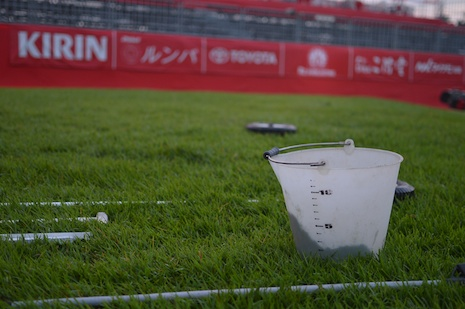
\includegraphics{img/b1-1.png}
\caption{A clipping bucket beside a putting green}
\end{figure}

Many golf courses in Japan track the volume of clippings mown off putting greens using this simple technique.\footnote{I wrote this blog post in August 2014 (\url{https://www.blog.asianturfgrass.com/2014/08/measuring-and-tracking-grass-clippings.html}). After the 2013 KBC Augusta tournament at Keya GC in Japan, Andrew identified a target clipping volume for the 2014 tournament, and I wrote about it in this post.} A plastic bucket is brought along on the mowing runs, the clippings are placed in the bucket, the bucket is shaken to allow the clippings to settle, and the volume of the clippings is recorded.

\begin{figure}
\centering
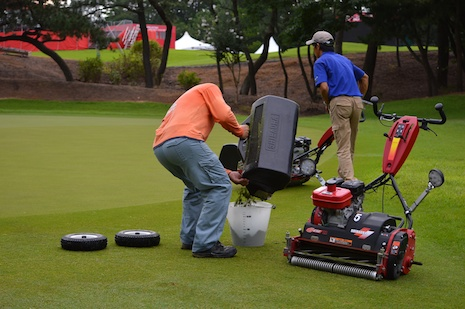
\includegraphics{img/b1-2.png}
\caption{Emptying mower clippings into a bucket}
\end{figure}

This information can be useful to check, track, and improve the management of putting greens, For example, the data can be used to:

ensure that all mowers are set up the same way

measure the effect of fertilizer applications

measure the influence of growth regulators

evaluate the effect of weather and maintenance practices on growth

track clipping yield for special events

\begin{figure}
\centering
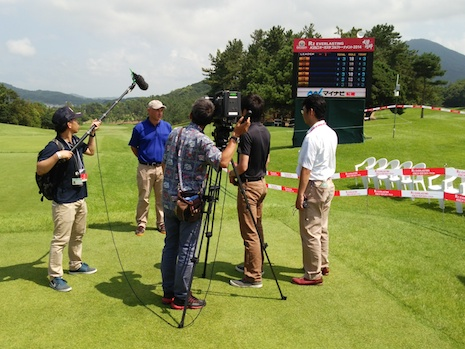
\includegraphics{img/b1-3.png}
\caption{Andrew McDaniel in an interview with a KBC television crew}
\end{figure}

Andrew McDaniel is the golf course superintendent at Keya GC in Fukuoka, where the Japan Golf Tour Organization (JGTO) holds the KBC Augusta tournament. Leading up to the tournament, the clipping volume of the korai (Zoysia matrella) greens was generally more than 20 L per day per green with a single cut. Today, on the Wednesday of tournament week, a double cut of the greens is collecting about 5 L of clippings per green. The progression to the tournament target clipping volume has been monitored carefully.

\begin{figure}
\centering
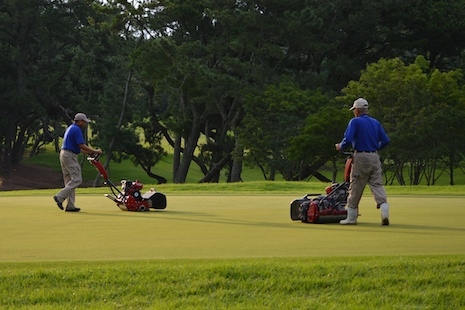
\includegraphics{img/b1-4.png}
\caption{Mowing the 1\textsuperscript{st} green at Keya GC during a practice round for the KBC Augusta tournament}
\end{figure}

He also used brushes on the mowers in the lead up to the tournament. When two mowers were used on the same green, each mowing the green once, the mower with the brush collected about twice as many clippings as the mower without the brush.~

For an even more detailed look at clipping production over time, and different ways I've seen it measured, see my report on clipping yield from putting greens (\url{http://www.seminar.asianturfgrass.com/20140612_clipping_yield.html}), which I've also reproduced as \protect\hyperlink{report2014}{Appendix C} at the end of this book.

\hypertarget{more-about-the-measurement-of-grass-clippings}{%
\chapter{More about the measurement of grass clippings}\label{more-about-the-measurement-of-grass-clippings}}

\begin{figure}
\centering
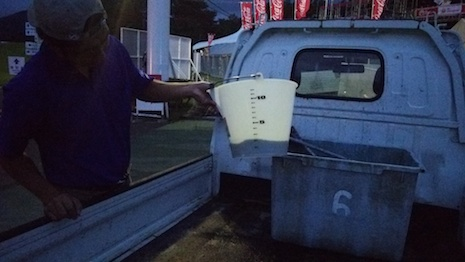
\includegraphics{img/b2-1.png}
\caption{Two liters of clippings from the putting green}
\end{figure}

One can measure the volume of clippings collected when mowing greens through the simple process of bringing along a bucket to empty the clippings into.\footnote{When I shared the information in the first chapter in 2014, there was a lot of discussion about this topic. I wrote this as a follow-up post a few days later (\url{https://www.blog.asianturfgrass.com/2014/08/more-about-the-measurement-of-grass-clippings.html}).}

This technique is used at Keya GC in Fukuoka, the host club for this week's KBC Augusta tournament. The greensmowers bring along a bucket and take note of the volume of clippings collected from each green.

\begin{figure}
\centering
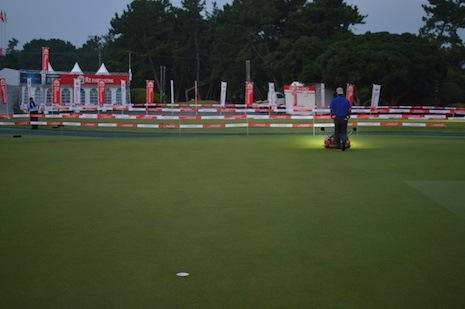
\includegraphics{img/b2-2.png}
\caption{Mowing the practice putting greens at Keya GC}
\end{figure}

In a previous post, I mentioned some of the ways that this information can be put to use. Here at Keya, the target for tournament week was to be at less than 10 L per green. During the 2013 tournament, the clipping volume averaged 11.8 L per green during tournament week, and 5.3 L per green in the week immediately after tournament week. The course superintendent, Andrew McDaniel, thought that putting surfaces for the 2014 tournament would be best if the clipping volume were slightly less than in 2013.

The clipping volume is collected year round, and from most of the greens. I've taken a subset of the 2014 data and plotted it for the month of August, with the average clipping volume from greens 1, 2, and 4, just to show how the yield has been this month, through this morning, the 2nd round of the tournament.

\begin{figure}
\centering
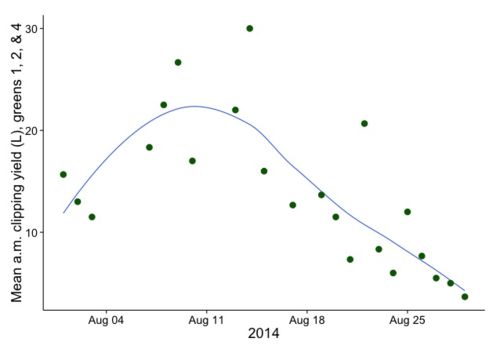
\includegraphics{img/b2-3.png}
\caption{August 2014 clipping volume from three greens at Keya GC}
\end{figure}

It looks like the clipping yield is close to the target range. By tracking the amount of clippings, one can adjust nitrogen rate, growth regulator applications, and mowing height and amount of mowing in order to modify the amount of clippings.

The use (or not) of brushes, or groomers, or the effects of various other maintenance practices can be evaluated when the clipping volume data are available. The Shibaura G-EXE22 mowers used on the greens can be fitted with this brush.

\begin{figure}
\centering
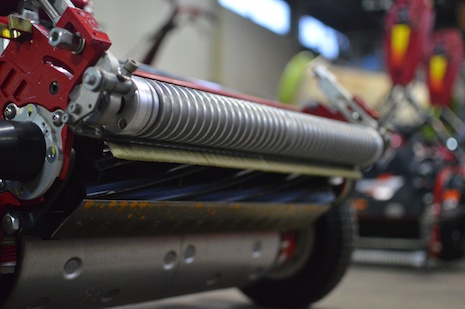
\includegraphics{img/b2-4.png}
\caption{Brush fitted between the front roller and the bedknife on the Shibaura G-EXE22}
\end{figure}

Andrew found that use of the brush increased the number of clippings by a factor of 2. During the tournament, the brushes are not being used, but in the lead up to the tournament, the brushes were used to increase the amount of clippings and help create the desired surfaces.

\begin{figure}
\centering
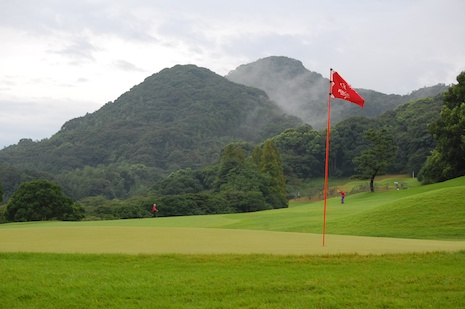
\includegraphics{img/b2-5.png}
\caption{View from behind the 14\textsuperscript{th} green at Keya GC}
\end{figure}

Now, during tournament week, the korai (Zoysia matrella) greens at Keya GC are growing at just the desired rate, and the mowers are removing the targeted amount of clippings. It doesn't take much extra time to collect this information, and having a time series of these clipping volume data can help a turf manager make decisions about the adjustments to make in green maintenance.

\begin{figure}
\centering
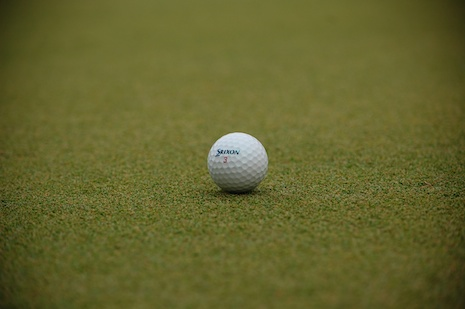
\includegraphics{img/b2-6.png}
\caption{Korai green surface at Keya GC}
\end{figure}

\hypertarget{clipping-volume-or-clipping-weight}{%
\chapter{Clipping volume, or clipping weight?}\label{clipping-volume-or-clipping-weight}}

The standard for measuring how much a turf sward is growing is to take the dry weight of the clippings mown off the turf.\footnote{I wrote this blog post in July 2017 (\url{http://www.asianturfgrass.com/2017-07-04-volume-or-weight/}).} This isn't a realistic option for routine turf management because who has drying ovens? And who can take the time to separate sand from clippings to reduce measurement error \citep{kreuser2011}? I find it easiest to measure the volume of the clippings. That's a fast and easy way to measure the clippings. I don't like fresh weight as much as volume, because fresh weight requires a scale, has the same problems with sand contamination, and some variation based on water in the samples that I suspect is higher with weight than with volume.\footnote{Jared Nemitz and Adam Moeller have shared information in articles and videos about regular measurement of fresh weight. This video, ``How It's Done: Measuring Clipping Yield From Putting Greens'' (\url{https://youtu.be/QtgwEqYmV6A}), and the ``Improving Management by Collecting Data'' case study (\url{http://archive.lib.msu.edu/tic/usgamisc/cs/275023.pdf}) describe how fresh clipping weight is measured from the 10\textsuperscript{th} green at the Peninsula Club at each mowing, and explain how that information is put to use \citep{nemitz2016}.}

\begin{figure}
\centering
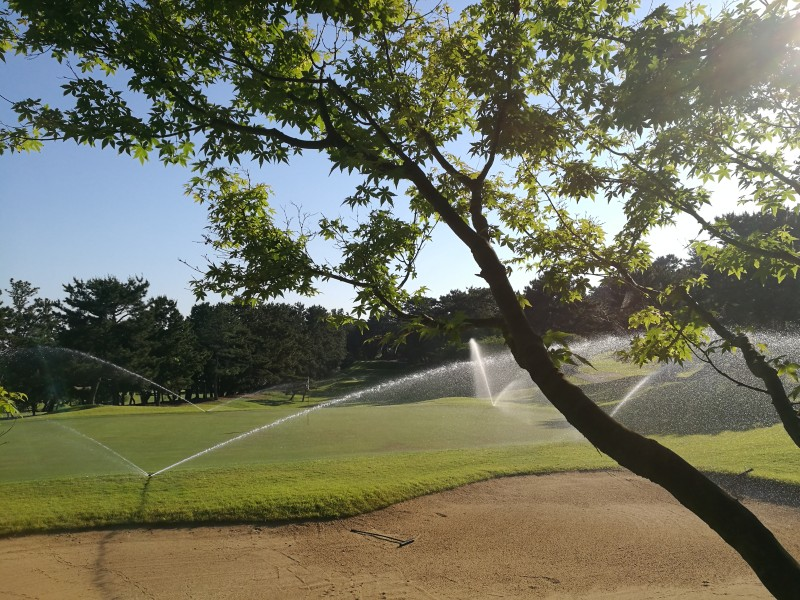
\includegraphics{img/keya_8_maple.jpg}
\caption{An \emph{Acer palmatum} in spring and a korai putting green in Fukuoka}
\end{figure}

I was at Keya GC in Fukuoka in late May. On three of the greens at Keya, the volume and the fresh weight of the clippings are measured. I don't recommend this! The only reason the maintenance staff are collecting these data are at my request, as part of a research project.

On May 29, sand topdressing was applied to the greens.

\begin{figure}
\centering
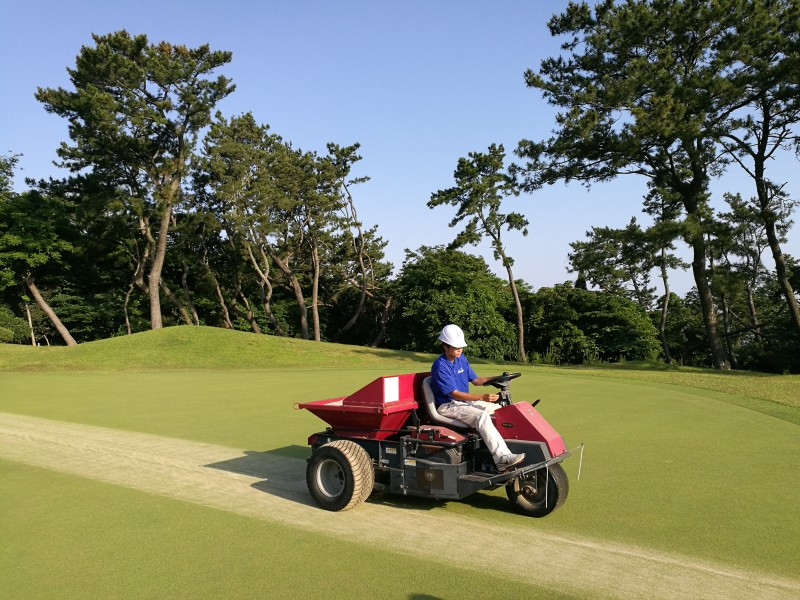
\includegraphics{img/keya_1_topdress.jpg}
\caption{sand topdressing application to the 1\textsuperscript{st} green at Keya GC}
\end{figure}

So what happened after that topdressing? Mowing was skipped for a few days. When mowing resumed, see how the ratio of fresh weight to volume spiked? And then took over a week to get back down to what it was prior to topdressing?

\begin{figure}
\centering
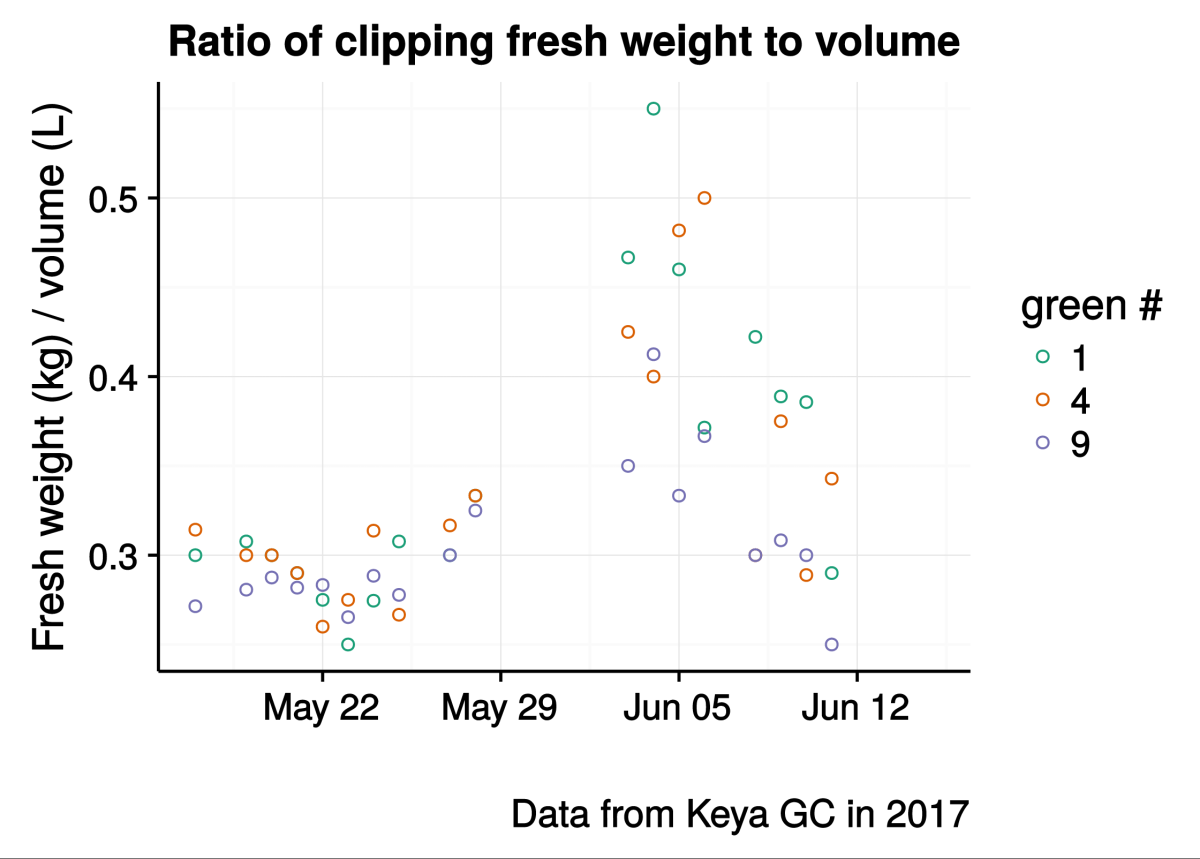
\includegraphics{img/ratioChart.png}
\caption{Ratio of clipping fresh weight to volume and the change after sand topdressing application}
\end{figure}

That's the effect of sand contamination in the samples, and it is one of the reasons I prefer routine tracking of clipping volume to the tracking of clipping mass.

\hypertarget{unitsChapter}{%
\chapter{Units of measurement}\label{unitsChapter}}

\hypertarget{note-about-units}{%
\section{Note about units}\label{note-about-units}}

You'll find various units of volume in this book. My first serious interest in this topic began at Keya GC in Fukuoka in 2013. At that time, I was thinking, and writing about clipping volume, in terms of liters per green.

That's fine for a single location; if one knows the green sizes and what a normal or target clippin volume is for a particular green, then that is the easiest way to think about it. In fact, I still think about it this way today, but I don't communicate it that way anymore. That's because there are different green sizes, or fairway sizes, or portions of a sports field, or lawn sizes, or whatever one is measuring. For communication about clipping volume to people at another property, or to estimate a dry harvest yield, it is necessary to express the volume in terms of area.

In Japan it is common to express this in terms of liters collected per 100 m\textsuperscript{2} (L/100 m\textsuperscript{2}).\footnote{The unit of L/100 m\textsuperscript{2} is roughly equivalent to quarts/1000 ft\textsuperscript{2}.} This measure works great for monthly totals. It would be common to have a monthly clipping volume from putting greens of 30 to 120 L/100 m\textsuperscript{2}.

For daily clipping volume, however, one ends up using a lot of decimal points when expressing in these units. When I wrote a report about this in 2017, this chart \protect\hyperlink{volHistogram}{reproduced in Appendix A} shows a median clipping volume of 1.2 L/100 m\textsuperscript{2} and 50\% of the measurements in a range from 0.67 to 2.2 L/100 m\textsuperscript{2}. It's not ideal to try to express the clipping volume and be using so many decimal points. It may be 1.2 today, 0.9 tomorrow, 0.8 the next day, skip a day of mowing because of rain, and then get 1.7.

This past winter I started expressing daily totals in units of mL/m\textsuperscript{2} which I much prefer, as explained in the next section.

And as for this book? Well, it is a work in progress. I'm going to convert all the units and charts to the units I'm using now. But for now, I'm publishing what I have.

\hypertarget{something-new}{%
\section[Something new]{\texorpdfstring{Something new\footnote{This is from a blog post in March 2018 (\url{https://www.asianturfgrass.com/2018-03-25-clipping-volume-green-speed-and-units/}), in which I explained that I would start expressing clipping volume in units of mL/m\textsuperscript{2} rather than the unit of L/100 m\textsuperscript{2} that I had used previously.}}{Something new}}\label{something-new}}

First, the new. I am going to start using a standard unit of mL/m2 to express the clipping volume. This is milliliters per square meter. I have previously used units of L/100 m2. This is an easy change to make. 1 L/100 m2 is 10 mL/m2.

Why the change? Because this gives a number for almost all measurements that will be between 0 and 100. Vigorously growing turf may be from 20 to 50 mL/m2. Haven't mown for a few days? You may get more than 50 mL/m2. Under tournament conditions, one might have less than 10 mL/m2 from a double cut of the surfaces. Using a unit on a scale from 0 to 100 is easier because it avoids decimal points. And it expresses the volume per square meter, which is the base area unit I prefer.

When I was in graduate school, I read a paper \citep{monteith1984} by John Monteith (\url{https://en.wikipedia.org/wiki/John_Monteith})---you'll recognize that name from the ``Penman-Monteith'' equation for evapotranspiration---entitled
\emph{Consistency and convenience in the choice of units for agricultural science}. Here's his advice:

\begin{quote}
``How should an appropriate multiple or sub-multiple of a unit be chosen? When repeated measurements of a quantity are to be reported, it is worth looking carefully for a unit which will avoid the frequent quotation of unnecessary zeros or decimal points. For example, the mean weight of a cereal grain should obviously be reported as 38.2 mg rather than 0.0382 g or 38200 μg. In general, when a quantity is quoted to two or more significant figures, the choice of unit should preferably allow its numerical component to fall between 1 and 100; but when only one significant figure is available, it should normally lie between 1 and 10.''
\end{quote}

I try to work with units that fall in that range, and I intend to start doing so in my discussion of clipping volume.

\hypertarget{measuring-clipping-yield-from-putting-greens}{%
\chapter{Measuring clipping yield from putting greens}\label{measuring-clipping-yield-from-putting-greens}}

Greenkeeping, at its core, is about controlling the growth rate of the grass.\footnote{This chapter was originally published in a slightly different form in my \emph{GCM China} column in 2015 (\url{https://www.blog.asianturfgrass.com/2015/07/an-easy-technique-for-monitoring-the-growth-rate.html}), and it was published again as a chapter in the \emph{Short Grammar} (\url{https://leanpub.com/short_grammar_of_greenkeeping}).} To get the desired green speed, or the maximum disease resistance, or the fastest divot recovery without too much thatch production, one must adjust the growth rate of the grass. An easy technique to monitor the growth rate is to measure the clipping yield from golf course putting greens.

\begin{figure}
\centering
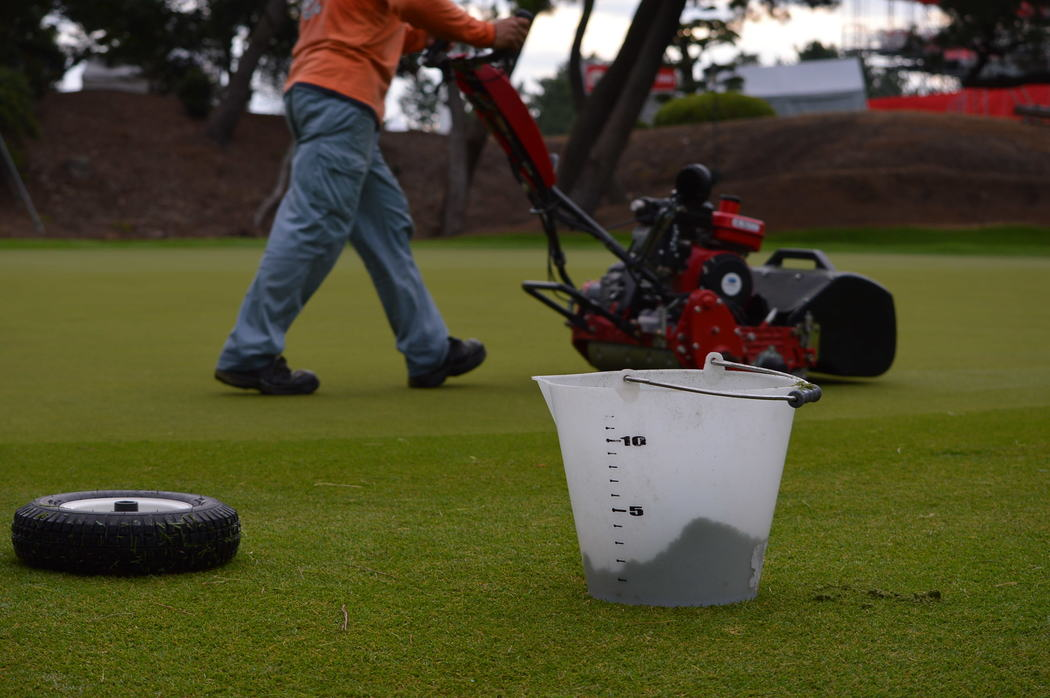
\includegraphics{img/b9-1.jpg}
\caption{Using a bucket to measure the volume of clippings from a single mow of a putting green}
\end{figure}

All that is required to do this is a plastic bucket with volume marks on the side. The person mowing greens can empty the clippings into the bucket, shake until the clippings are level, and then record how many liters of clippings were mown from the green. It is customary to correct the clipping yield for the size of the green, expressing the clipping yield as volume per area. I prefer units of mL/m\textsuperscript{2} for daily and monthly measurements, and L/m\textsuperscript{2} for annual totals. See the \protect\hyperlink{unitsChapter}{Units of measurement} for more about this.

Why might one want to do this? These data on clipping yield can be used for a number of things. Because different mowers are usually used on the course, it can be useful to check the yield across the course to find out if all the mowers are set up in the same way. By measuring the clipping yield, one can track the effect of fertilizer applications, and get some idea of when the growth rate changes and fertilizer re-application may be required.

One can also use these data to measure the influence of plant growth regulators such as trinexapac-ethyl, to evaluate the effect of weather and maintenance practices on growth, to see if greens situated in different microclimates have different growth rates, and to track clipping yield for special events. For example, under tournament conditions it is usually desirable to have a very slow growth rate, because that leads to more consistent conditions through the day. Also, when the grass is growing slowly, the greens have the potential to be faster.

I don't know what the normal amount of clippings will be for any golf course. That depends on the season and the type of grass and on the desired growth rate. A busy course needs to have a faster growth rate, to recover from traffic damage. A course without much play doesn't need as much growth. Let's say that the normal growth rate at a golf course is 50 mL/m\textsuperscript{2}/d. During a tournament, the ball may roll better through the day if the clipping yield is less than 10 mL/m\textsuperscript{2}/d. By tracking how the clipping yield changes and how fertilizer and irrigation and plant growth regulators affect the clipping yield, one can prepare for special events or tournaments with consistency and precision.

There are other ways to measure clipping yield too -- measuring the mass of clippings is one way, and keeping track of the number of times the mower baskets need to be emptied is another. I think the easiest and most consistent way to measure as part of routine golf course maintenance is to note the volume of clippings.

\hypertarget{tournament-week-clipping-volume}{%
\chapter{Tournament week clipping volume}\label{tournament-week-clipping-volume}}

\begin{figure}
\centering
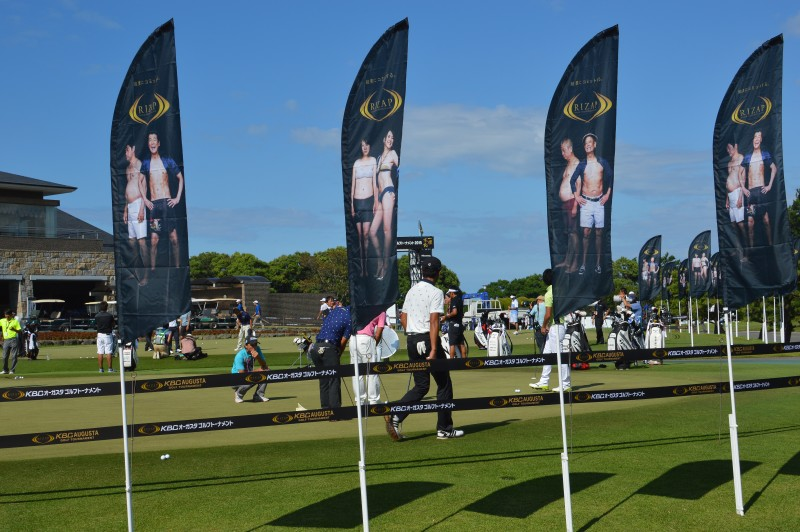
\includegraphics{img/b4-1.jpg}
\caption{Practice putting greens during the 2015 KBC Augusta Tournament}
\end{figure}

The KBC Augusta golf tournament is held the last week of August at Keya Golf Club near Fukuoka.\footnote{I wrote this on the ATC blog after the 2015 KBC Augusta tournament (\url{https://www.blog.asianturfgrass.com/2015/09/tournament-week-clipping-volume.html}). By this time, I was really starting to see how useful this measurement was, and just how repeatable the numbers were, and especially, just how \emph{easy} it was to get such a valuable measure of how much the grass is growing.} The greens are korai (Zoysia matrella) and when the greens are mown, the volume of clippings is noted.

\begin{figure}
\centering
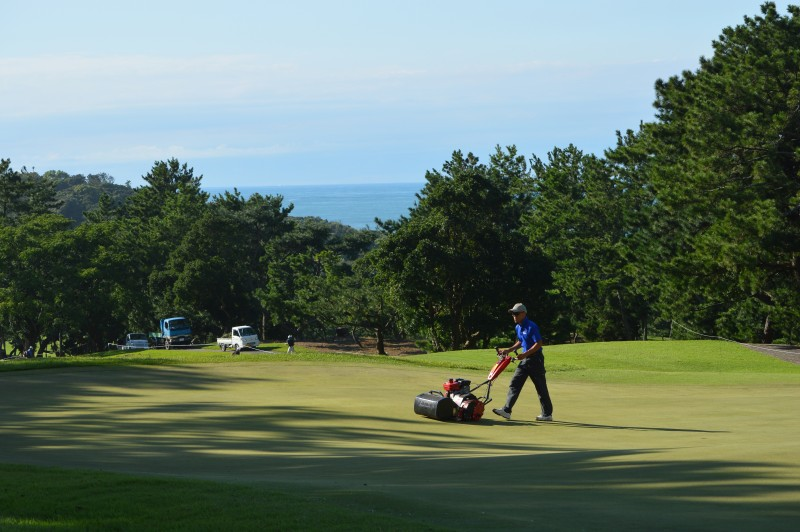
\includegraphics{img/b4-2.jpg}
\caption{Mowing the 16\textsuperscript{th} green at Keya GC; the volume of clippings will be measured when the mower basket is emptied}
\end{figure}

These data are collected not only during the tournament week, but throughout the year when the greens are mown.

\begin{figure}
\centering
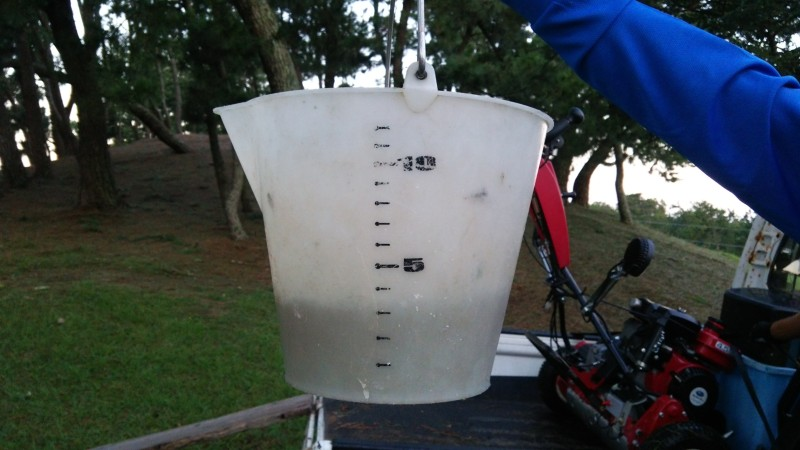
\includegraphics{img/b4-3.jpg}
\caption{A bucket graduated in liters used for measuring clipping volume}
\end{figure}

Andrew McDaniel, the greenkeeper at Keya GC, shared the clipping yield data with me and I've summarized it in these charts.

The average daily clipping yield, plotted week by week through the year, shows that the grass starts growing at the end of March, reaches a peak in the hottest weather of July and August, before dropping down due to tournament preparations. This reduction in clipping volume is achieved by reducing the N rate, only adding irrigation to prevent dry spots, and applying trinexapac-ethyl.

\begin{figure}
\centering
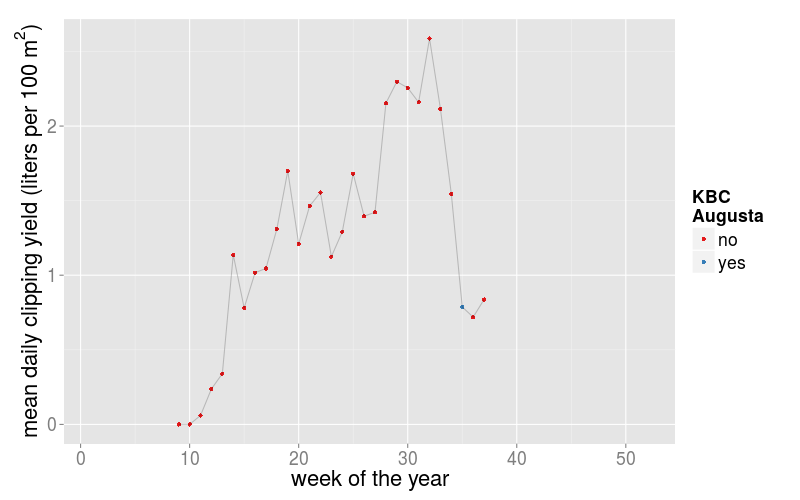
\includegraphics{img/b4-4.png}
\caption{Keya GC mean daily clipping volume by week in 2015}
\end{figure}

Looking just at August of 2015, one sees there were 4 days when the greens could not be cut due to heavy rain. One of those days was 25 August, the Tuesday of tournament week, when a typhoon came through. Not surprisingly, the clipping volume is larger on the day after a missed mowing.

\begin{figure}
\centering
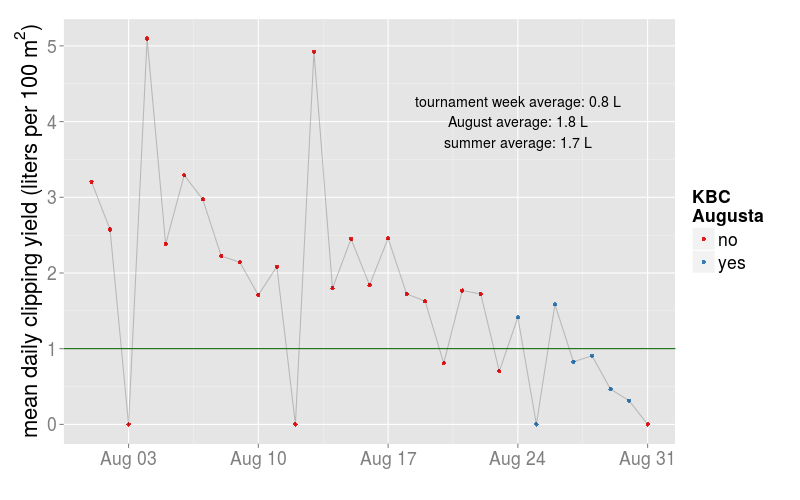
\includegraphics{img/b4-5.png}
\caption{Keya GC mean daily clipping volume in August 2015}
\end{figure}

There was a downward trend through August, with the maintenance being done in a way that targets a clipping yield during tournament week of less than 1 liter per 100 m2 of green area.

Looking at clipping volume every day in 2015, it is even more clear when the grass starts growing in the spring, and also that the korai doesn't really grow until after the rainy season, when the temperatures increase. It is only in July and August when the grass is growing quickly. This chart also shows the days during the season when the greens could not be mown.

\begin{figure}
\centering
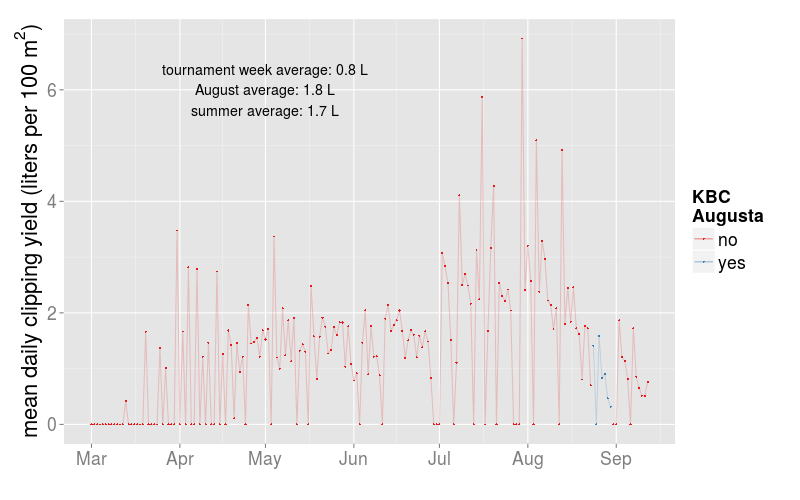
\includegraphics{img/b4-6.png}
\caption{Keya GC mean daily clipping volume in 2015}
\end{figure}

Looking at clipping volume for the 2013, 2014, and 2015 KBC August tournaments, one can see the 2014 and 2015 tournaments had less than 1 liter per 100 m2 from Thursday through Sunday. Based on measurements of green speed and evaluation of ball roll, the goal in 2016 will be to get the clipping yield down to the 1 liter level by the start of tournament week.

\begin{figure}
\centering
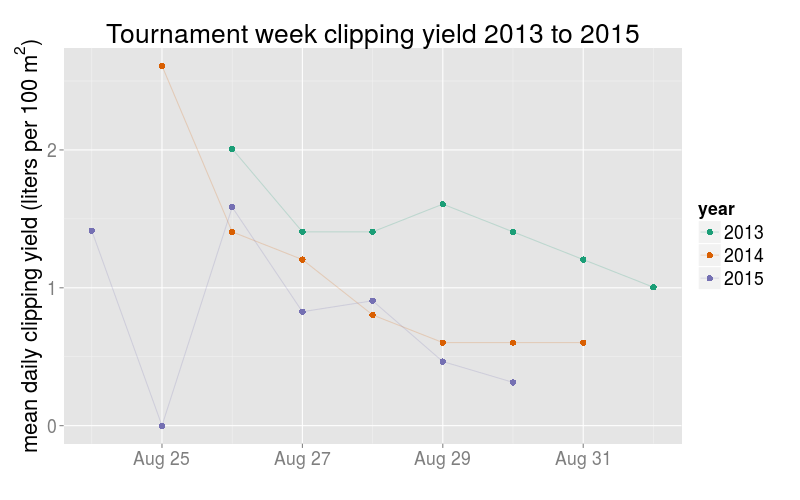
\includegraphics{img/b4-7.png}
\caption{Clipping volume from the 2013 to 2015 KBC Augusta tournaments}
\end{figure}

These measurements don't take much time to collect and they can be useful in evaluating how the maintenance work should be adjusted to achieve the desired green conditions.

\begin{figure}
\centering
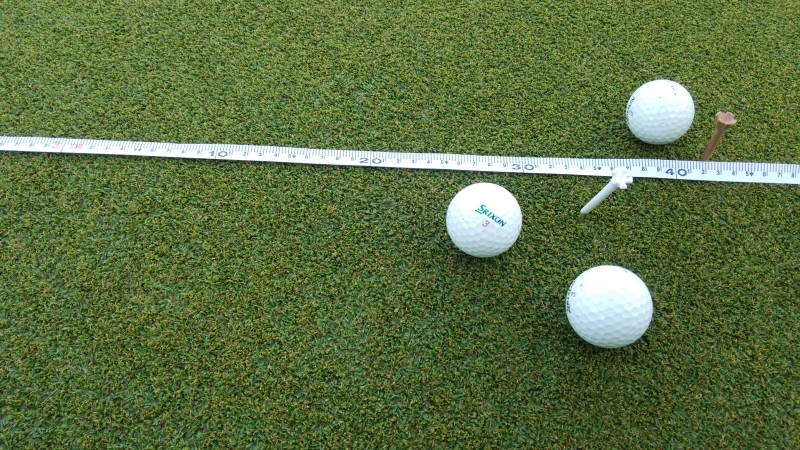
\includegraphics{img/b4-8.jpg}
\caption{Golf balls and a measuring tape on a korai putting green during the KBC Augusta tournament}
\end{figure}

What about the work that was done to get this clipping volume, and the conditions produced?

\begin{itemize}
\tightlist
\item
  On the greens at Keya GC, 8.5 g N and 3.5 g K/m2 since the start of 2015.
\item
  Mowing height for the tournament was 2.6 mm with the Shibaura 22 inch GEXE.
\item
  Except when adjusted due to weather, the greens were mown 2x each morning, then rolled with a Toro lightweight roller, and then were mown 1x at the end of the day.
\item
  Primo Maxx and soil surfactants applied to the greens.
\item
  Irrigation added as necessary to prevent dry spots.
\item
  Morning green speed during the tournament rounds ranged from 10.7 to 11.2 feet.
\end{itemize}

\hypertarget{clipping-volume-variation-from-green-to-green}{%
\chapter{Clipping volume variation from green to green}\label{clipping-volume-variation-from-green-to-green}}

Ryo Ishikawa won the KBC Augusta tournament at Keya GC in Fukuoka this week.\footnote{I wrote this post (\url{https://www.blog.asianturfgrass.com/2016/08/clipping-volume-variation-from-green-to-green.html}) immediately after the 2016 KBC Augusta tournament.} Before the tournament started, he was so struck by the green conditions that he wrote about it on his website.\footnote{You can read an English translation of his post at the start of the article about Andrew McDaniel from \emph{Golf Digest}, kindly translated by Yukio Ueno and available at \url{http://www.files.asianturfgrass.com/andrew_digest_2018.html}.}

\begin{figure}
\centering

\includegraphics{img/b3-1.png}
\caption{Ryo Ishikawa's message on his website}
\end{figure}

During the tournament, he putted well, with 27 putts Thursday, 26 Friday, 24 Saturday, and 26 Sunday. He had no three putts and 41 one putts on these korai greens during the tournament.

The greenkeeping staff at Keya GC measure the volume of clippings from 12 greens when the greens are mown. I shared some photos of this process, and some of the results during the tournament this year, in a series of tweets during the 2016 tournament. These tweets have been organized into this Twitter moment, and you can view them all in one place here: \url{https://twitter.com/i/moments/990124653527023616}.

I wondered how the clipping volume at Keya GC during the tournament this year compared to other courses. I also wondered if the variation in clipping volume from green to green during the tournament was different from clipping volume variability during a regular week.

To do that, I looked at clipping volume from 7 consecutive days in which greens were mown. Data from Keya during tournament week in 2016 are in the chart below, along with data from the last 7 mowing days at Keya during July 2016, and data from earlier this year from two different courses with cool-season grass.

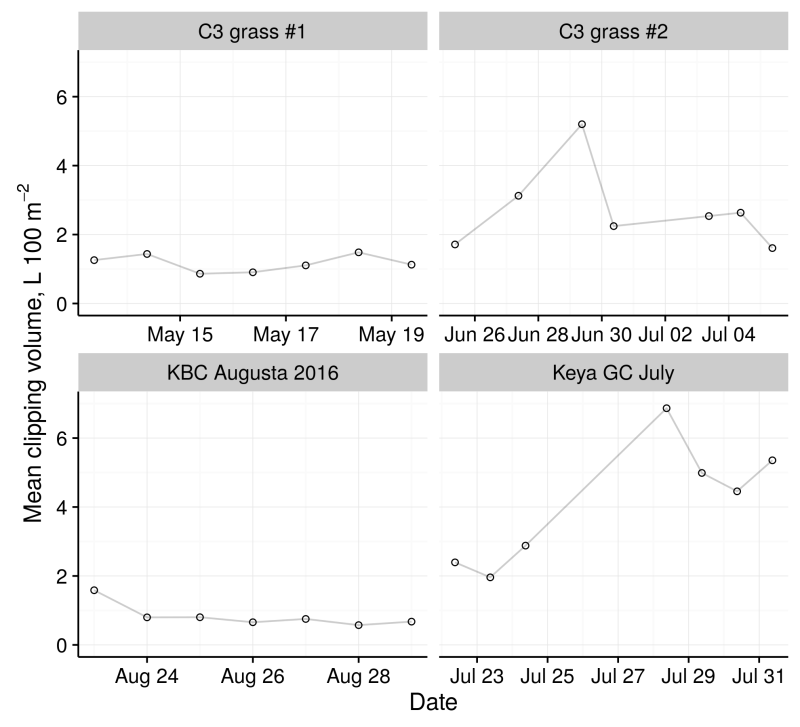
\includegraphics{img/b3-2.png}

As far as consistency in the volume of clippings, the tournament data looks impressive. I would expect that this consistency in clipping volume would result in more consistent ball roll on the greens during a tournament compared to everyday play.

I wanted to look also at the variability in clipping volume from green to green on a particular day.\footnote{In this post I was looking at the coefficient of variation. I now am less interested in looking at the coefficient of variation and think it is more useful to look at the standard deviation of clipping volume data as an indication of variability. The C\textsubscript{v} gets really low when the clipping volume is high, even where there is quite a lot of variation.} Is the variability in clipping volume from green to green lower during the tournament maintenance? To do that, I calculated the coefficient of variation (cv) for these same data. The cv is the standard deviation (σ) divided by the mean (μ).

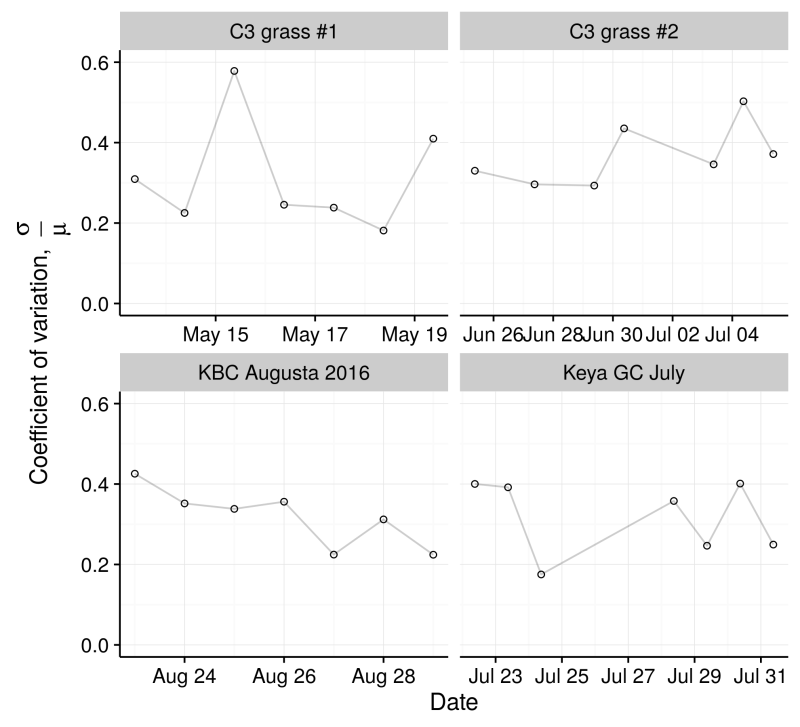
\includegraphics{img/b3-3.png}

I like that the cv during the tournament week was on a downward trend. I don't see a huge difference in the overall cv -- the mean cv for these dates is 0.31 for C3 grass \#1, 0.37 for C3 grass \#2, 0.32 for Keya at KBC Augusta 2016, and 0.32 for Keya during the last 7 mows of July.

One might speculate that greens with the same growing environment and the same soil and the same grass would have a lower cv. The cv shown here may represent some indication of the microclimate effect on growth across a property.

\hypertarget{already-proving-to-be-more-valuable-that-i-originally-expected}{%
\chapter{``Already proving to be more valuable that I originally expected''}\label{already-proving-to-be-more-valuable-that-i-originally-expected}}

\begin{figure}
\centering
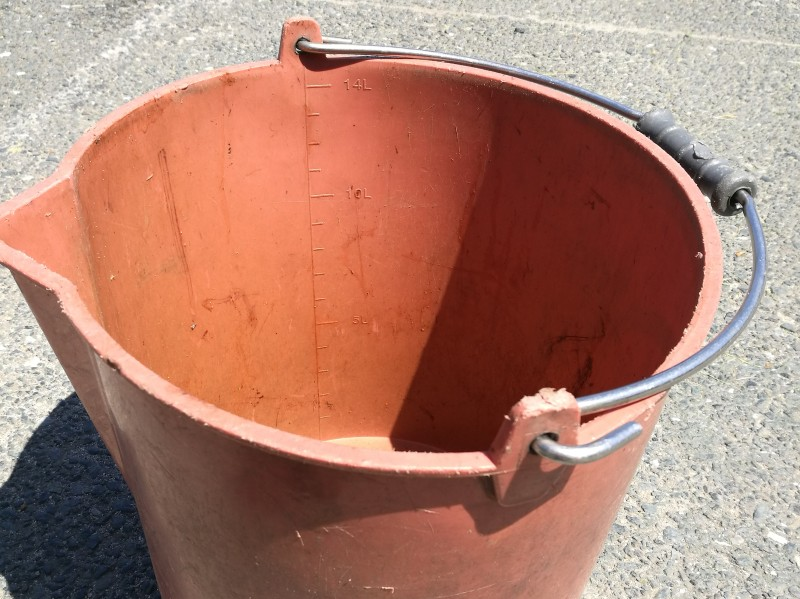
\includegraphics{img/b5-1.jpg}
\caption{Another graduated bucket used to measure clipping volume from putting greens}
\end{figure}

When I read Jason Haines' interesting post about clipping yield, soil mineralization, and disease rates (\url{http://www.turfhacker.com/2017/06/growth-and-disease-rates.html}) and came to the part where he said measuring all the greens was more valuable than he expected, I was glad to read that.\footnote{This post was published on the ATC blog in 2017 at \url{https://www.blog.asianturfgrass.com/2017/06/already-proving-to-be-more-valuable-than-i-originally-expected.html}} I wanted to say ``I told you so,'' because this is a number that I think is really useful. And I hadn't thought of the disease connection and being able to notice that, but I do know that golf course superintendents will find ways that I haven't thought of to make use of growth data. Because managing the growth rate of the grass is what it all boils down to. I've written about this in the \emph{Short Grammar of Greenkeeping} (\url{https://leanpub.com/short_grammar_of_greenkeeping}). And it makes sense to me, when the clippings are collected anyway, why not take note of how many there are?

Chris Tritabaugh wrote about this on Twitter, \footnote{You can find that thread at \url{https://twitter.com/ct_turf/status/876765926347214848}} asking what about the fertilizer that wasn't applied? And he finds, if I understand correctly, that monitoring the clippings gives some confidence that more N \textbf{is required} or \textbf{is not required at a given time}.

Which is where I decide to jump in here with two quick comments. First, yesterday I had the great pleasure of writing about \emph{fertility} (\url{http://www.blog.asianturfgrass.com/2017/06/tonights-reading.html}). Now I want to mention \emph{programs}. Specifically, \emph{fertility programs}. I don't think program is the right word to use when considering the nutrient supply to turf.

Program means a plan of activities, or a sequence of operations that can be set to happen automatically. But with turfgrass, one can assess, as Chris wrote, ``the nutrients we haven't applied'' by measuring how much the grass is growing. That is, the grass is likely producing some growth in response to fertilizer applied in the past\footnote{See this post for more about that (\url{http://www.blog.asianturfgrass.com/2014/09/seasonal-nitrogen-use-how-much-and-when.html})} and one expects there is some growth related to mineralized N too.

Let's say one wants to have a flexible fertilizer system. FFS. Has a nice ring to it. Measuring the growth allows one to adjust the nutrient supply based on the grass response. Whatever one wants to call it, I think turf response will almost certainly be better, and fewer inputs will be required, if the N rate changes at almost every nutrient application. This is what the temperature-based growth potential method is based on, to set an upper limit of N supply at any time, given the weather, and then that predicted amount to supply is adjusted based on the actual grass response.

Now my second point, which is more about the utility of clipping volume. Or about mineralized N. One can expect a soil with a 10 cm rootzone depth and 1\% organic matter to release about 2 g N/m2 in a year. And a soil with 2\% OM may release about 4 g N/m2. For creeping bentgrass maintained at relatively low N, I expect that will produce from 50 to 100 g dried clippings per m2. And based on the relationship between clipping volume and dry weight for bentgrass, I expect that will work out to a fresh clipping harvest of 80 to 160 L/100 m2.

That is, one can predict how much extra the grass may grow after one knows the organic matter in the soil. I expect this makes sense to anyone who has put a number to the clippings mown off the putting greens, and is gibberish to everyone else. But the approach of working with quantities of nutrients in the soil, quantities of nutrients harvested, and quantities of nutrients supplied as fertilizer, allows one to get really precise, and really efficient, and supplying just what the grass requires.

And the implications are that one gets better grass conditions, one does so with less work, one has more control of the grass conditions, and there is potentially less coring, less topdressing, less disruption of surfaces, less \emph{Poa annua} invasion, etc.

\hypertarget{morning-clipping-volume-during-tournament-week-at-kbc-augusta}{%
\chapter{Morning clipping volume during tournament week at KBC Augusta}\label{morning-clipping-volume-during-tournament-week-at-kbc-augusta}}

The KBC Augusta tournament is coming up next week\footnote{I wrote this in mid-August 2017, just before the 2017 tournament (\url{https://www.asianturfgrass.com/2017-08-14-morning-clipping-volume/}).} at Keya Golf Club in Fukuoka. The volume of grass clippings cut from the greens is measured every morning.

I think it is interesting to look at the density\footnote{(\url{https://en.wikipedia.org/wiki/Probability_density_function})} of the measurements. This ridgeline plot\footnote{For more about this type of plot and what is being displayed, see the vignette (\url{https://cran.r-project.org/web/packages/ggridges/vignettes/introduction.html}).} provides a quick summary of clipping volume during the 2016 tournament.

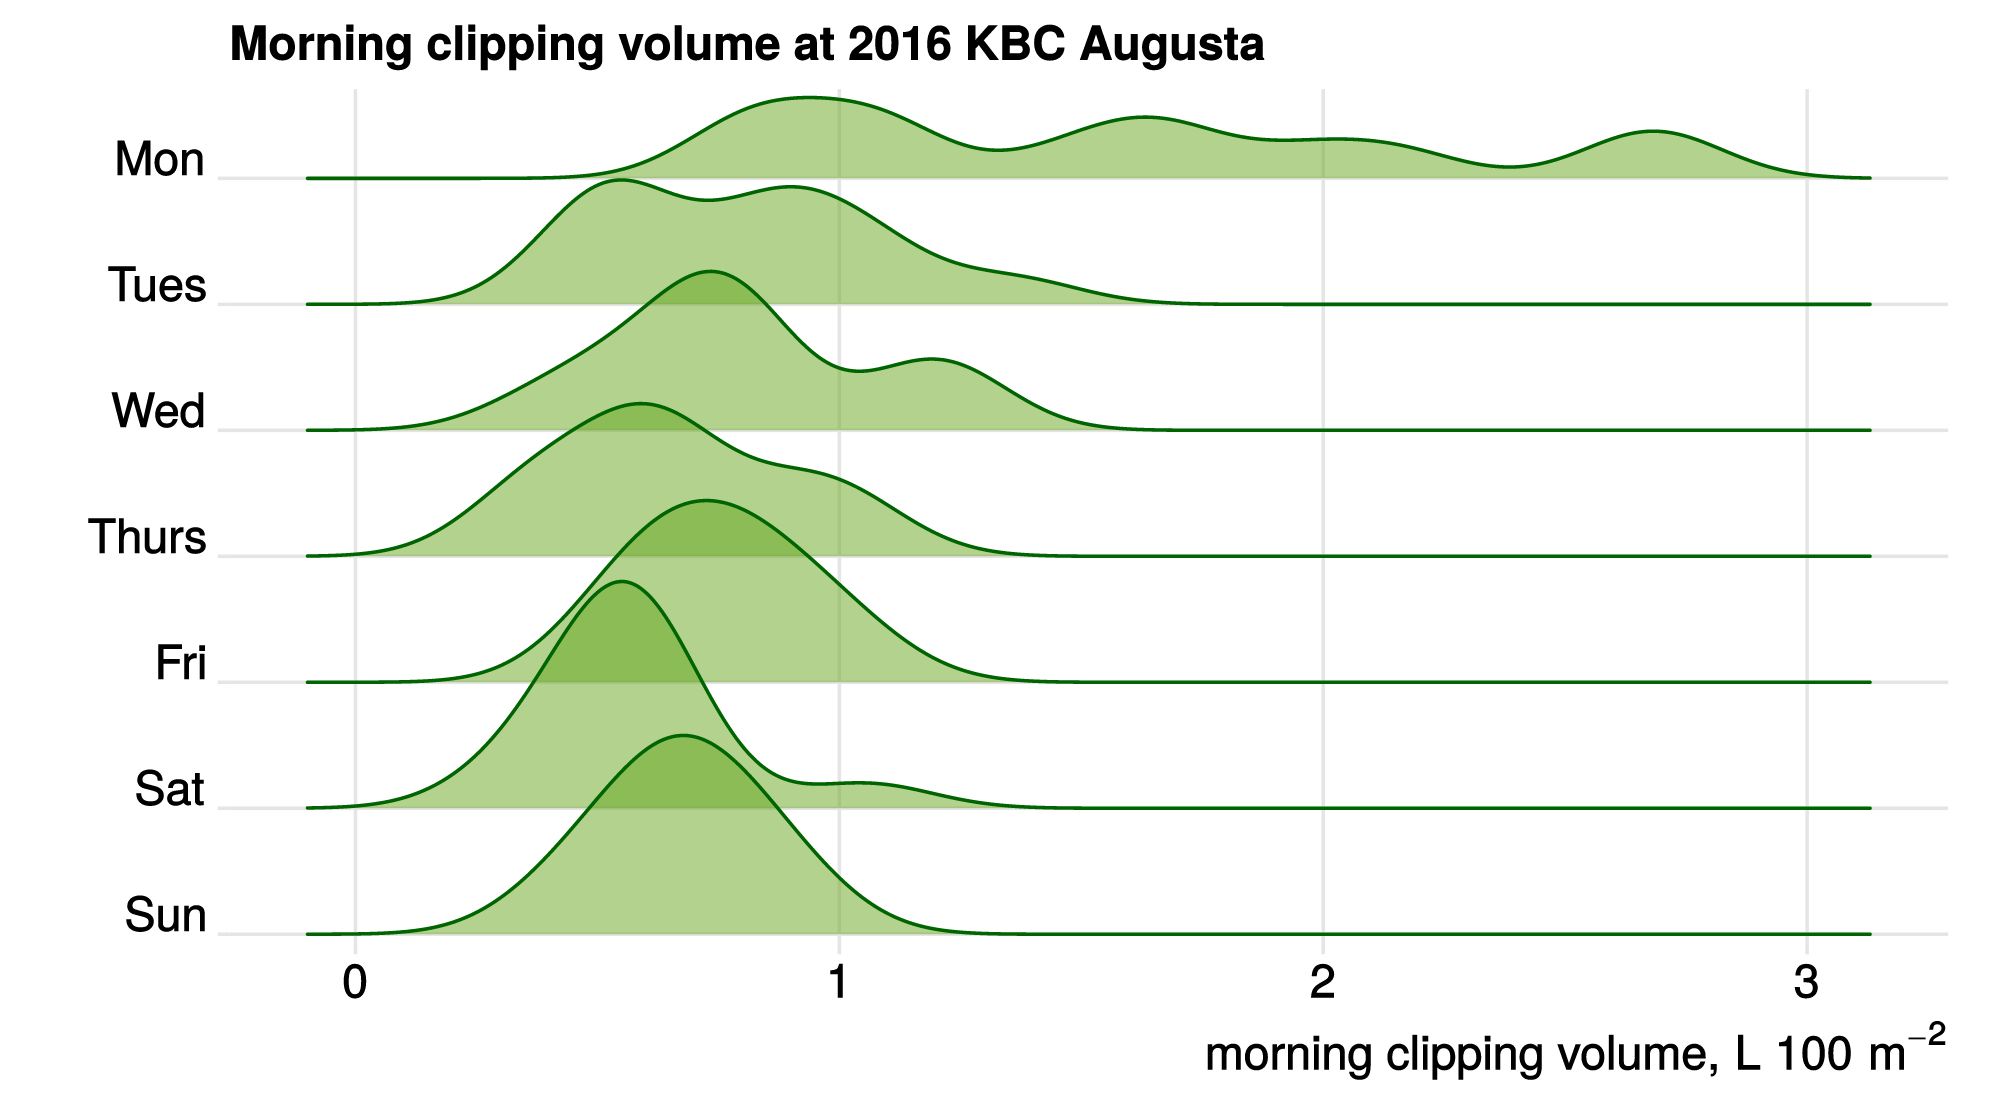
\includegraphics{img/b6-2.png}

The joyplot above uses the same data as this chart I made last year.

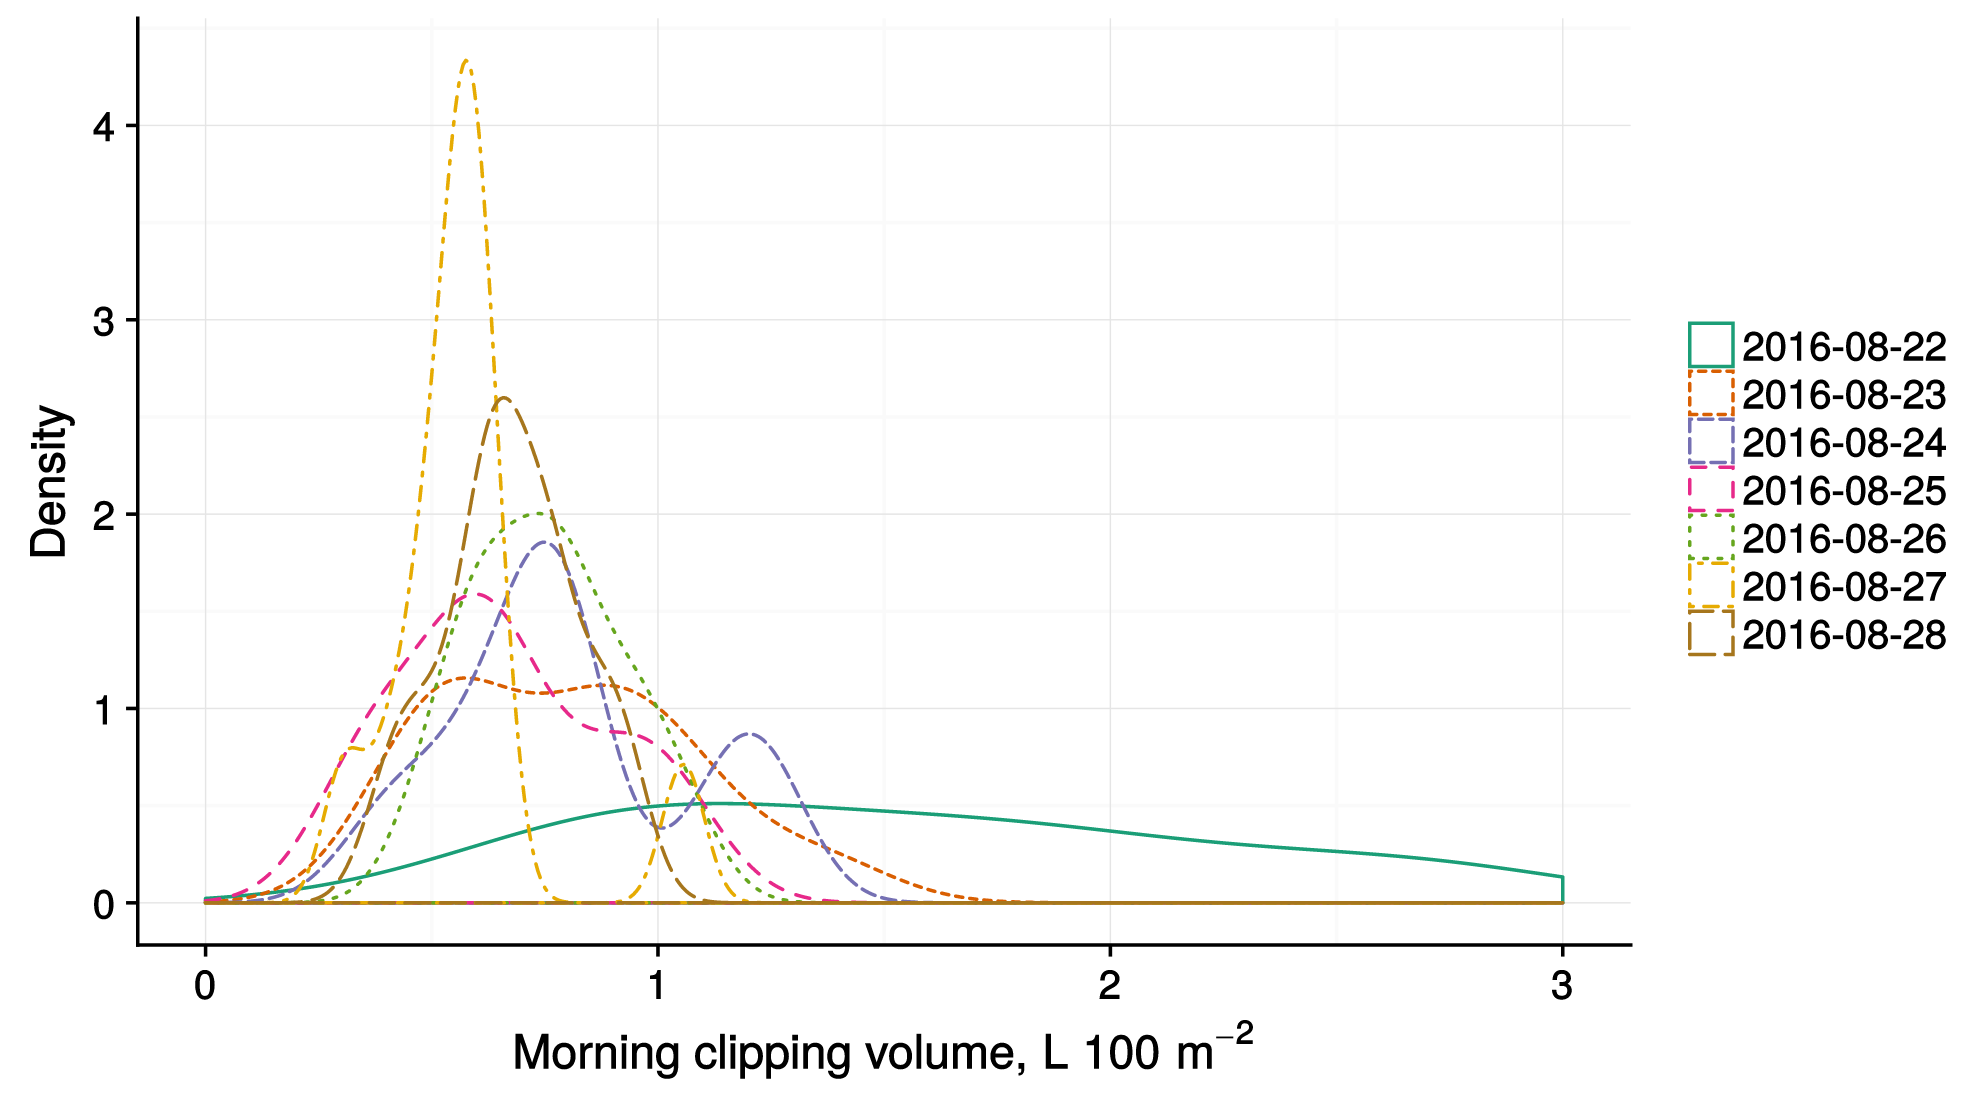
\includegraphics{img/b6-3.png}

\hypertarget{flipping-things-around}{%
\chapter{Flipping things around}\label{flipping-things-around}}

One can look at the growth of the grass, as approximated by the clipping volume, in a couple of ways. There's the quantity of clippings -- \emph{here's how much the grass is growing}. I think that's the typical way to look at it.

\begin{figure}
\centering
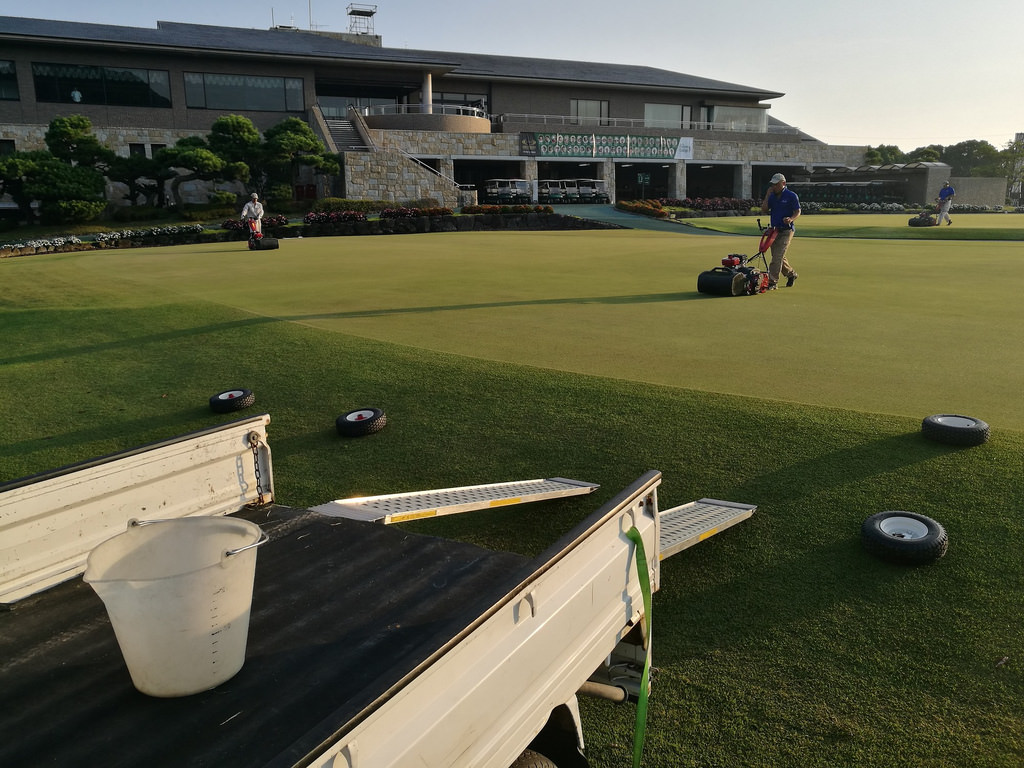
\includegraphics{img/b7-1.jpg}
\caption{Mowing practice greens at Keya GC}
\end{figure}

But I find it useful sometimes to flip things around,\footnote{This chapter is from a blog post I wrote in 2017 (\url{https://www.asianturfgrass.com/2017-09-15-flipping-things-around/}). Bob Raley wrote (\url{https://twitter.com/bobraley/status/909582862139224064}) to remind me that the efficiency of the fertilizer matters. As an example, 1 gram of N from urea is almost certainly going to produce more immediate growth than will 1 gram of N from an organic fertilizer. That's correct, and in this chapter I'm thinking more in terms of plant N use than I am fertilizer N supply. The topic of turfgrass growth, N use by the grass, and N supply to the grass from the soil and from fertilizer, is fascinating. I've been studying this and have a drafted but unpublished blog post in response to Bob's reply. By the way, Bob's article \citep{Raley2013} about N and P fertilizer and \emph{Poa annua} encroachment into a creeping bentgrass green is one that I take every chance to recommend. He measured an increase in \emph{Poa annua} when P fertilizer was applied. Here's a summary quote: ``Results of this study demonstrate that annual bluegrass encroachment into a newly established creeping bentgrass putting green can be curtailed by withholding P fertilizer such that soil P concentrations and P uptake are below levels that foster the competitive ability of annual bluegrass.'' If I were managing a mixed stand of creeping bentgrass and \emph{Poa annua} and wanted to favor the bentgrass, I would withhold P, and I would also use clipping volume measurements to find a target growth rate at which bentgrass grows more than \emph{Poa annua}.} and think about what produced that growth. Let's say for a particular turf area, for an upcoming event, I want to have a clipping volume of about 15 mL/m2/day (1.5 L/100 m\textsuperscript{2}/day). Let's say that's the amount of clippings I want to produce for a monthlong duration. That'll be about 450 mL/m\textsuperscript{2}/month (45 L/100 m2/month).

How much nitrogen (N) will it take to produce that much growth?

\begin{figure}
\centering
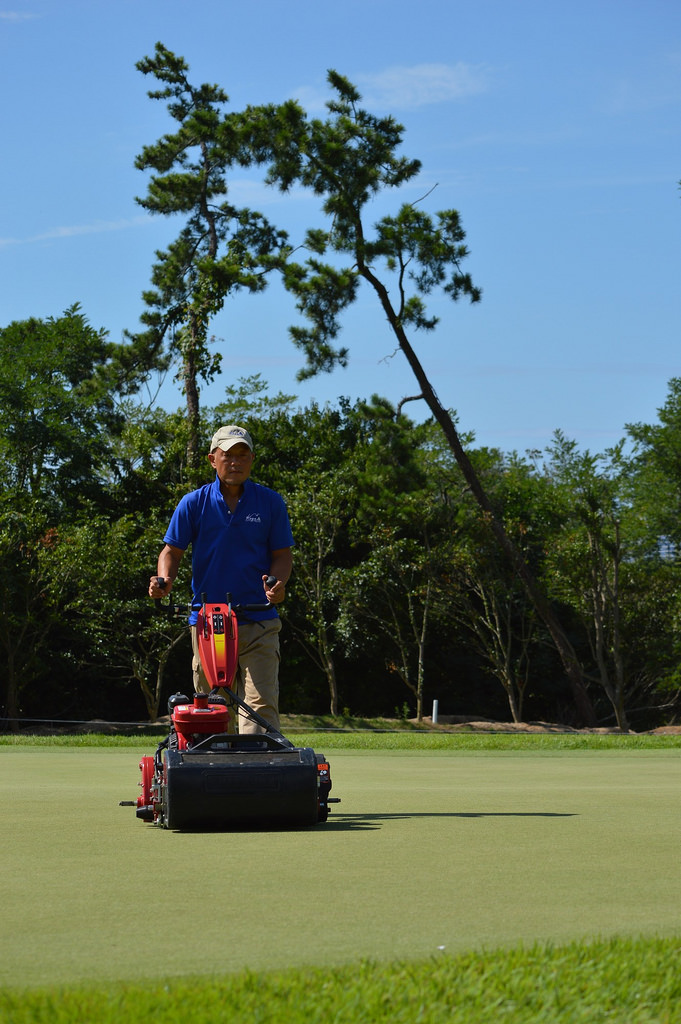
\includegraphics{img/b7-2.jpg}
\caption{Mowing the 2\textsuperscript{nd} green at Keya GC}
\end{figure}

For creeping bentgrass, I expect that will be just over 1 g N/m2. To get that much growth on korai (all the pictures in this post are korai), I expect the grass will use about 1.5 g N/m2.

\begin{figure}
\centering
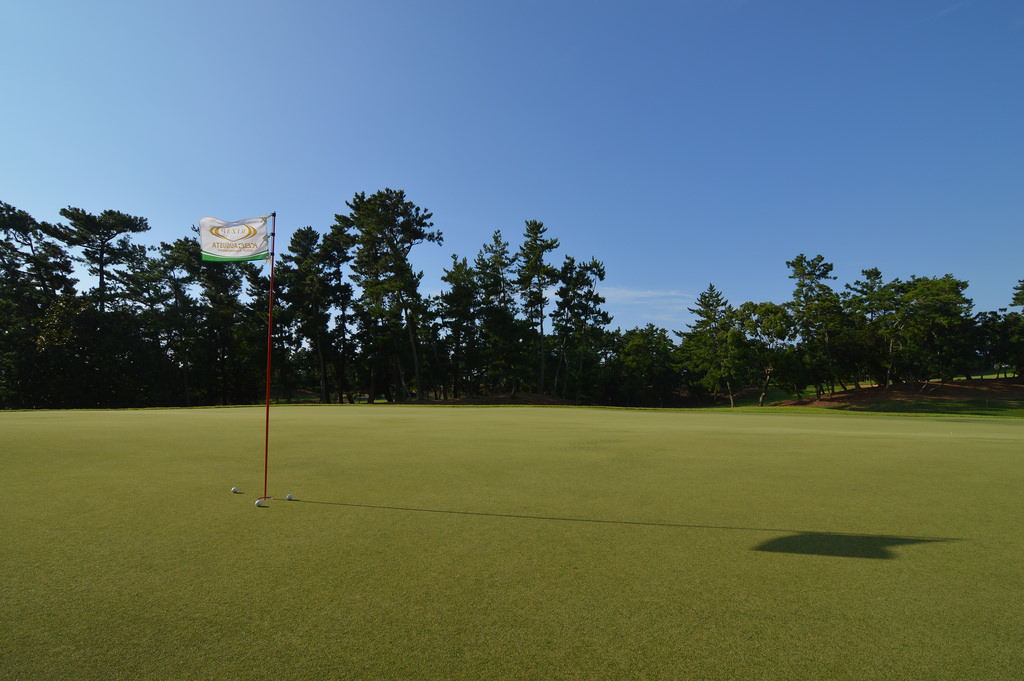
\includegraphics{img/b7-3.jpg}
\caption{The 5\textsuperscript{th} green at Keya GC}
\end{figure}

By knowing how much growth one wants, and about how much N it takes to produce that much growth, one can be a little more precise with the turf management.

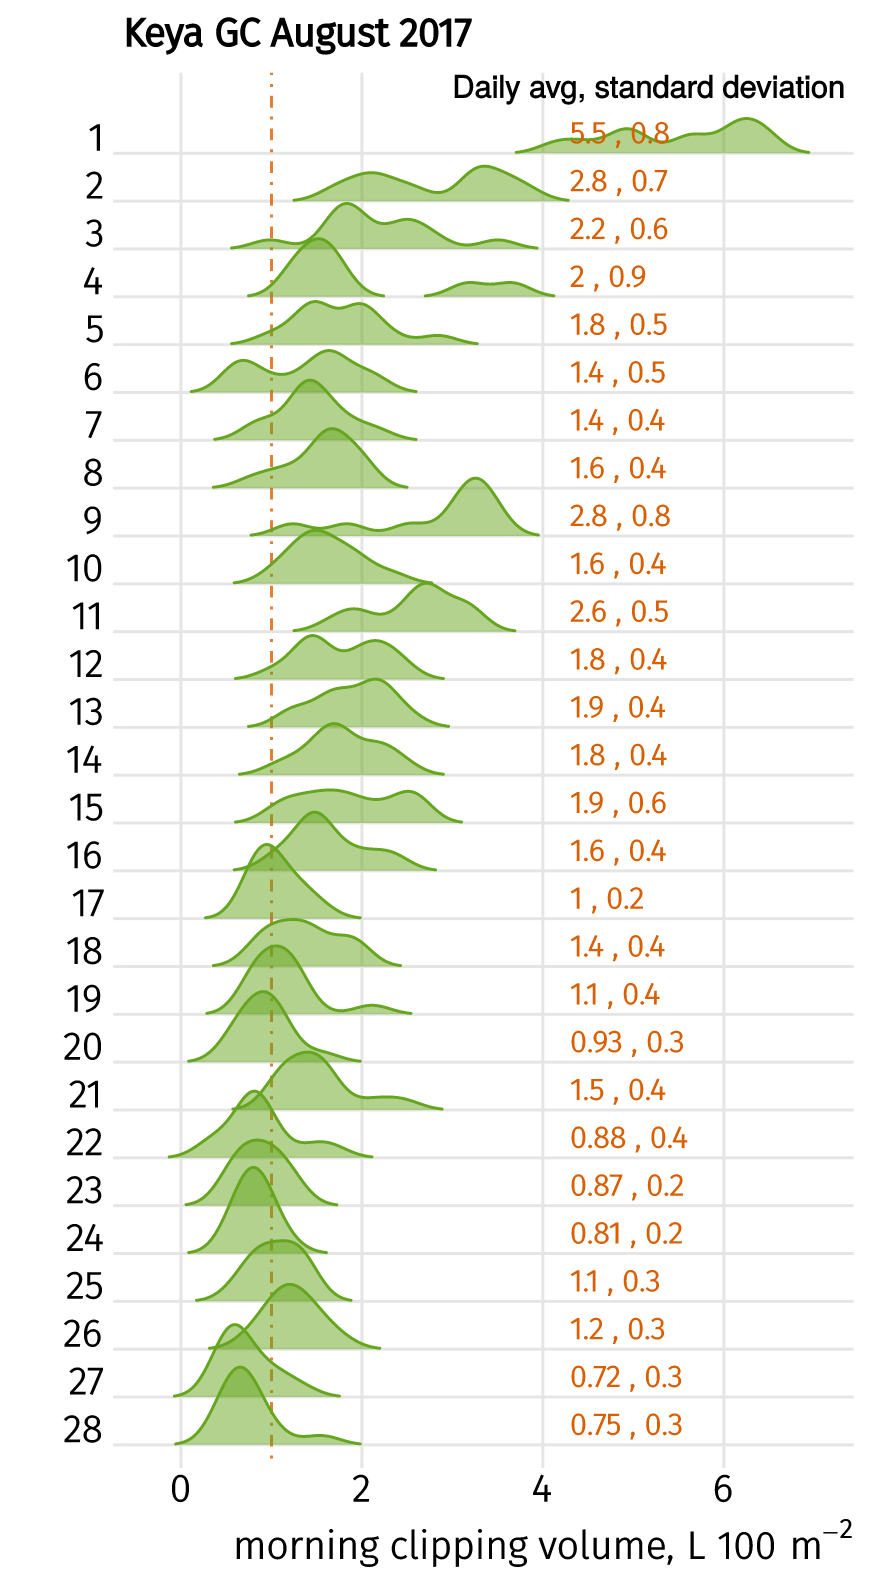
\includegraphics{img/b7-4.png}

\hypertarget{historical-clipping-data}{%
\chapter{Historical clipping data}\label{historical-clipping-data}}

It is really interesting, for me at least, to see how much grass grows. One way to put a number to how much grass grows is to measure the clipping volume of the grass mown from an area. With putting greens, for example, the baskets are going to be emptied anyway, so why not record how many clippings are in the baskets? It doesn't take much time.

After one has the measurement, it may look something like this.\footnote{I wrote about this in a blog post in the autumn of 2017 (\url{https://www.asianturfgrass.com/2017-10-13-clipping-vol-avg/}).} These are the clipping volumes for 19 greens (18 holes plus the practice green) on a golf course in Japan that was mown 189 out of 273 days from January 1 through September 30 in 2017.

\begin{figure}
\centering
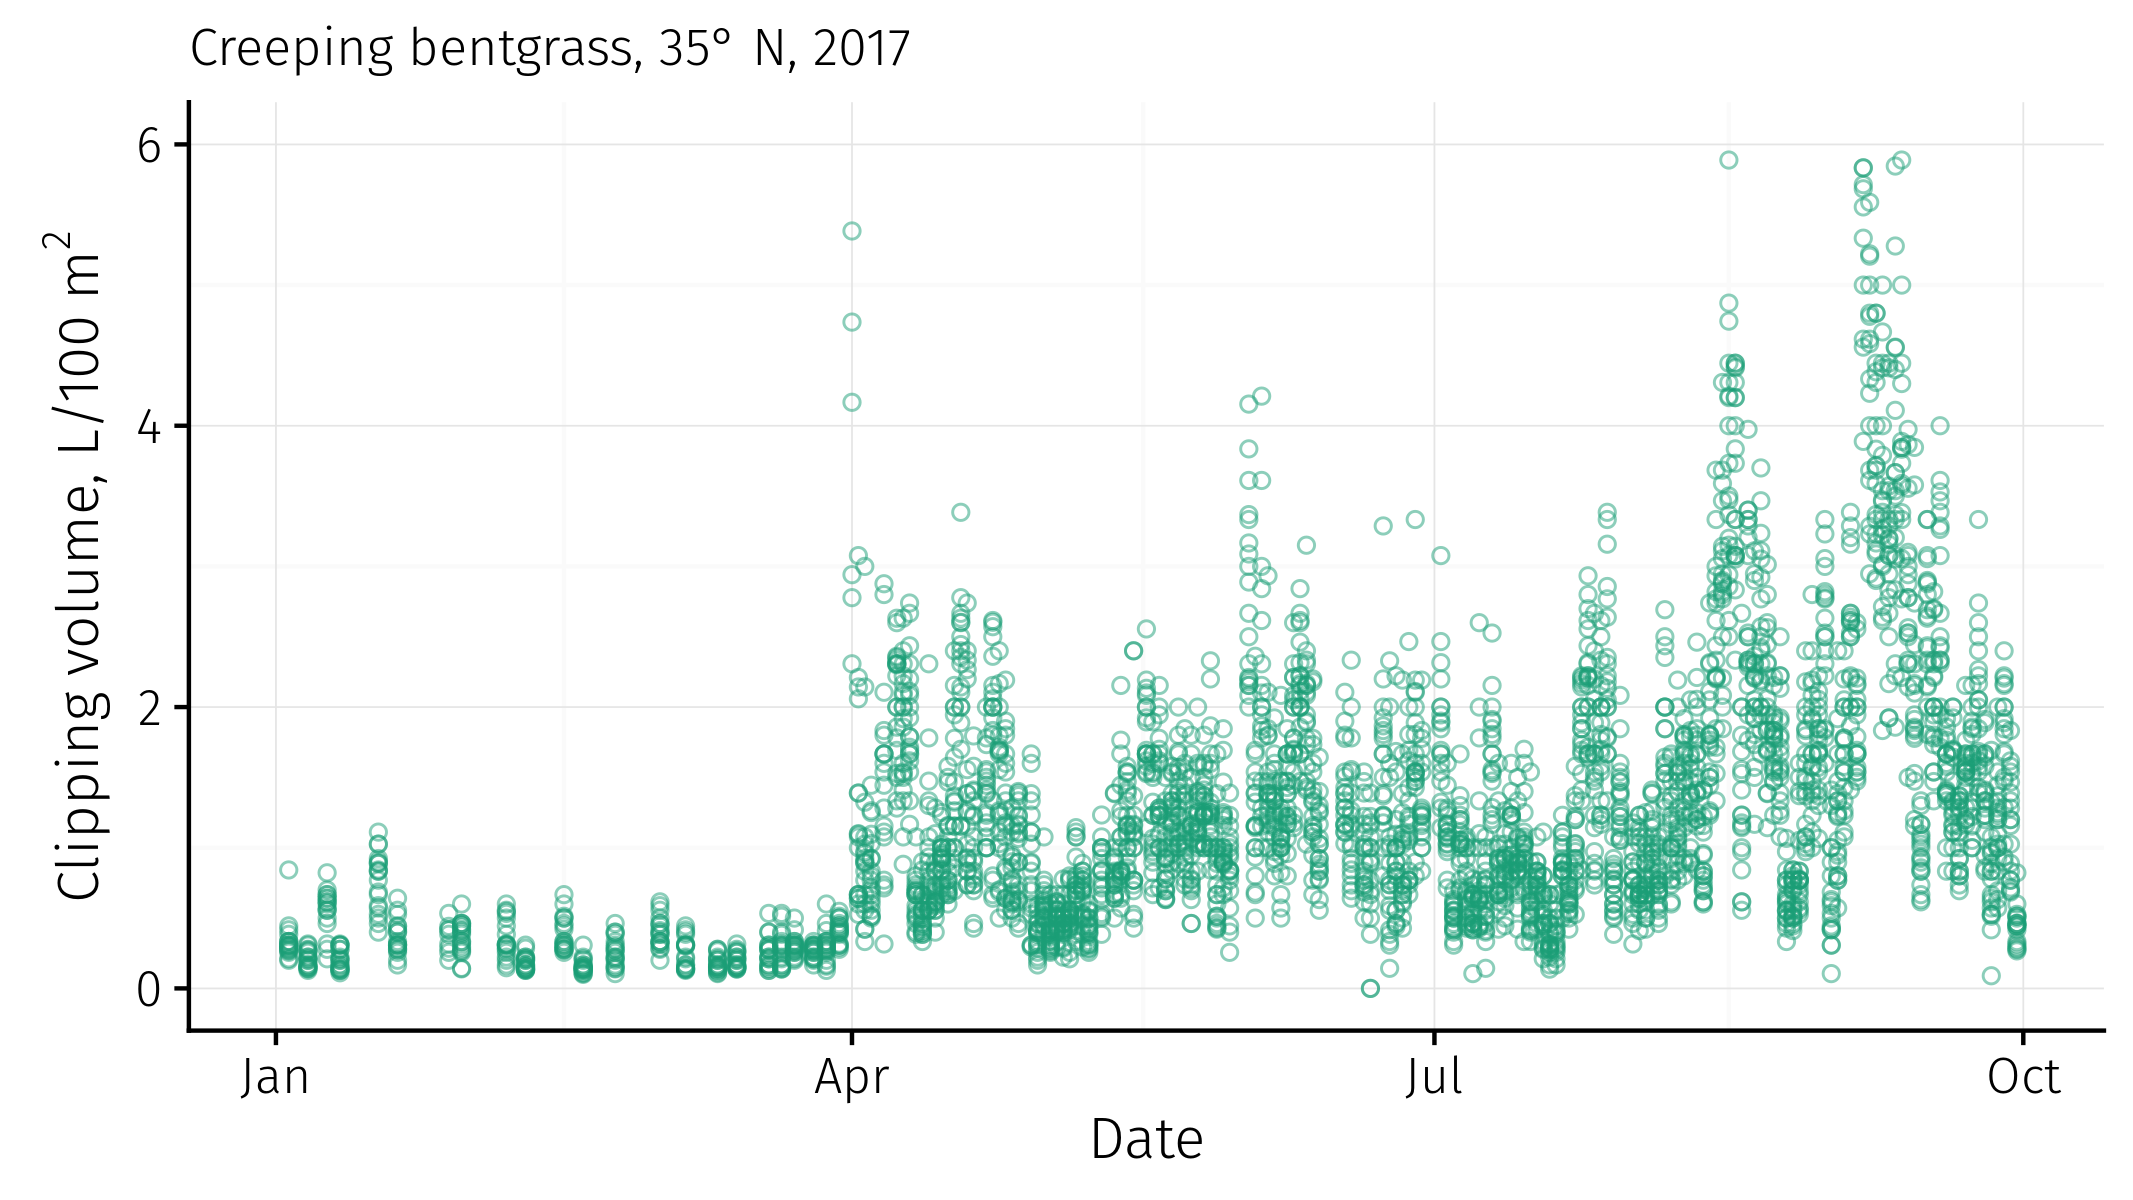
\includegraphics{img/b8-1.png}
\caption{Nine months of clipping volume data from 19 greens at one facility}
\end{figure}

Actually, that's a bit messy. One isn't going to be able to make many decisions from that set of data. And I only want to collect data if I can use it as a decision-making tool. Of course, having the measurements from multiple greens allows one to check the variability in clipping volume from green to green.

But what I'm most interested in is how much the grass is growing. To do that, I like to look at a moving average. This next chart takes the 189 days of mowing data this year and plots the daily average (from all 19 greens) and has a line showing the 5 day moving average (4 previous days, plus today, averaged).

\begin{figure}
\centering
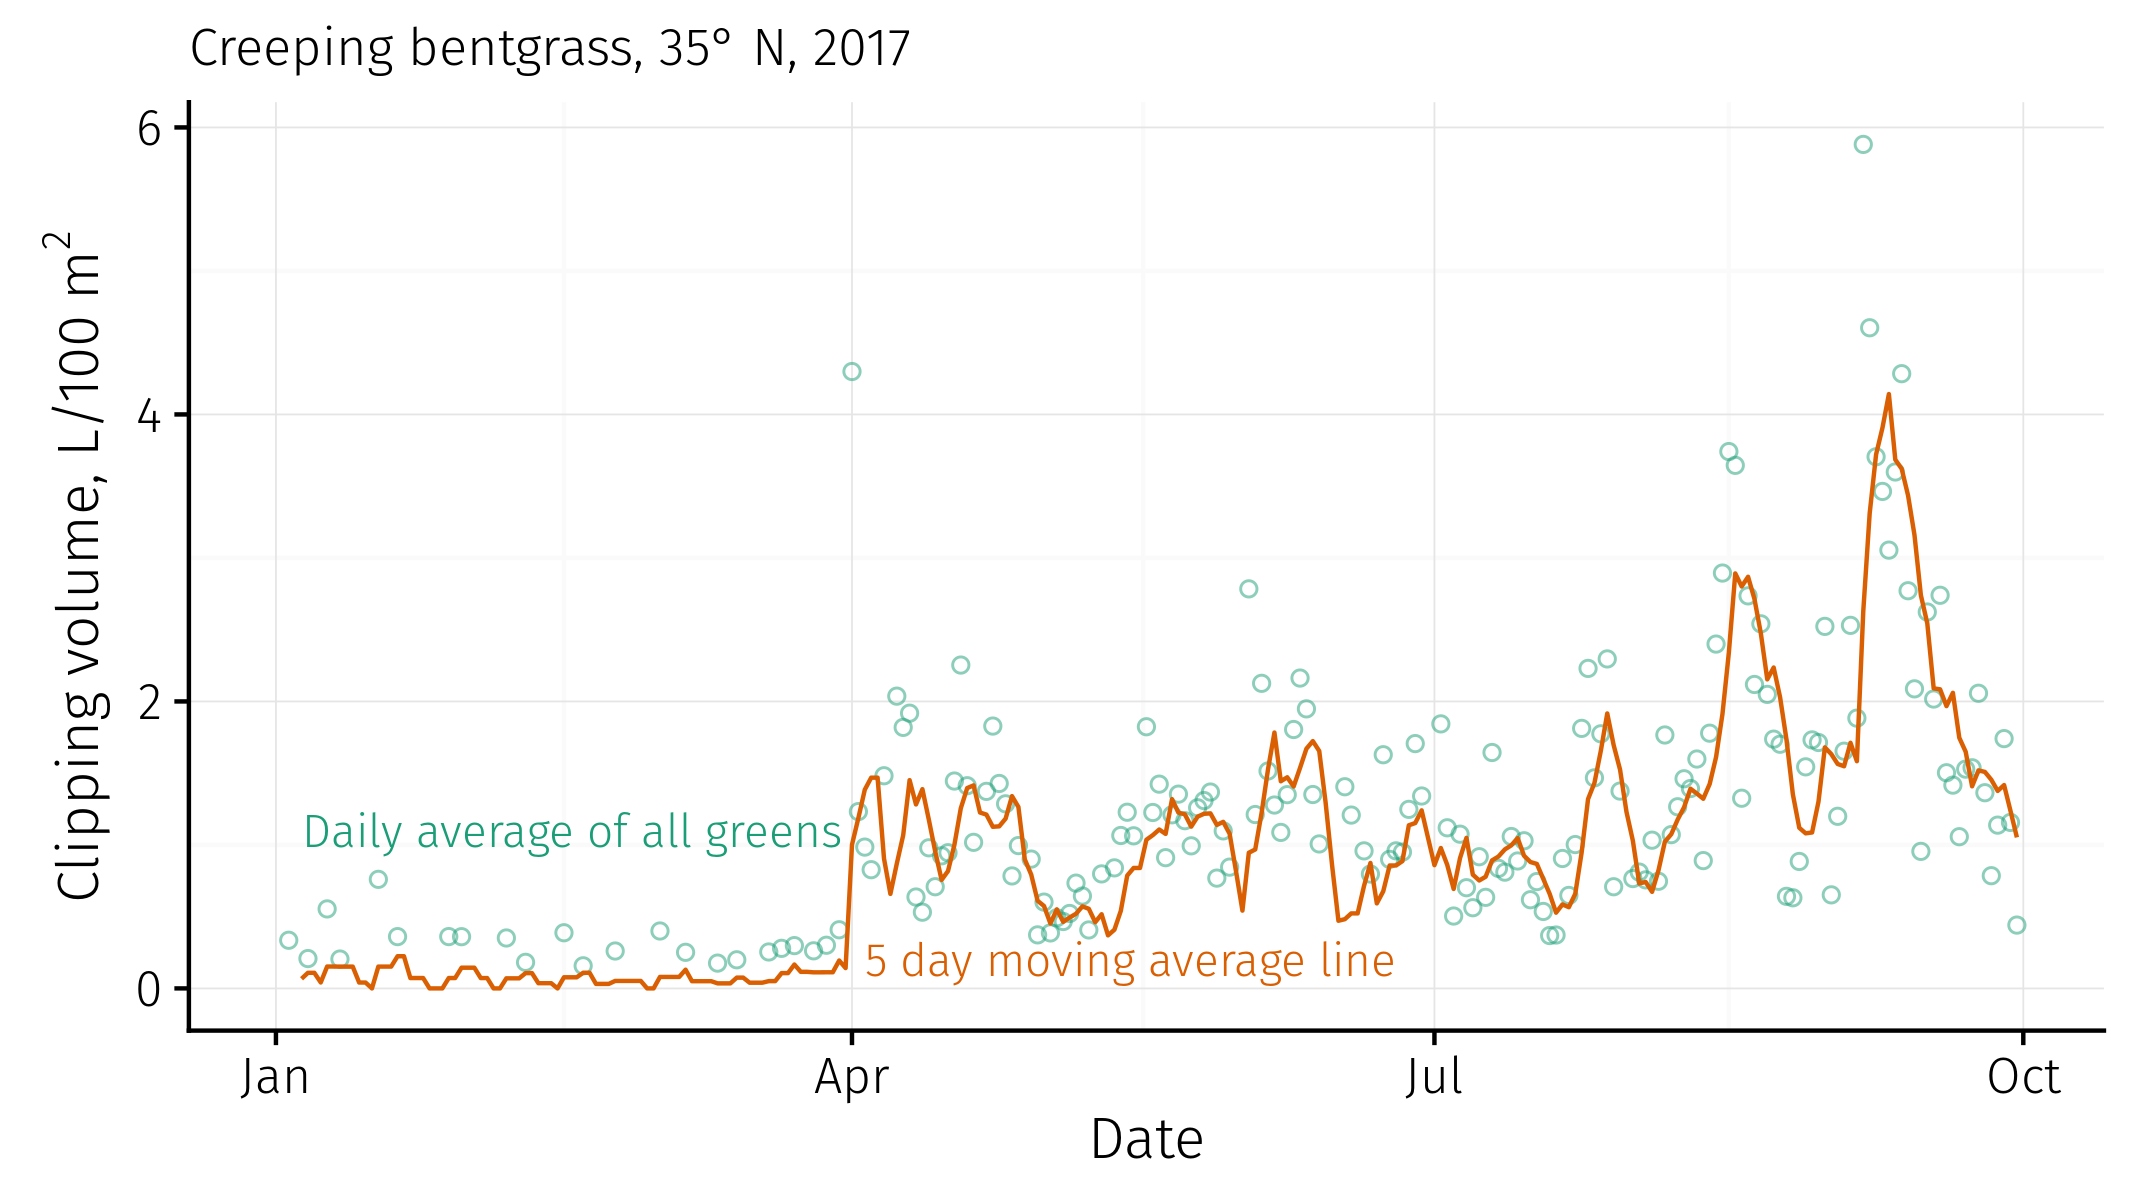
\includegraphics{img/b8-2.png}
\caption{The daily average and a five day moving average of clipping volume from 19 greens at one facility}
\end{figure}

The moving average seems easy to use as a decision making tool. What is the level of growth we have right now, as represented by the moving average, and is it moving in the direction I want it to be for tomorrow, next week, and next month? If it is, then I'll keep doing what I've been doing. If it isn't, then I'll make adjustments.

\hypertarget{animation1}{%
\chapter{Clipping volume timelines}\label{animation1}}

I made a chart\footnote{Early June 2018, that's when I put the post on this topic together (\url{https://www.asianturfgrass.com/2018-06-03-clipvol-animation-and-green-speed/}). This chapter is a substantial revision of that post, but the chart is the same.} to describe how I think of \#ClipVol.\footnote{The \#clipvol hashtag on Twitter (\url{https://twitter.com/hashtag/ClipVol?src=hash}) is a quick and easy way to see how turf managers are using this rapid measurement of turfgrass growth.}

This static version of the chart highlights a few of the things I look at. An animated version is at \url{https://www.asianturfgrass.com/img/y2018.gif}.

\begin{figure}
\centering
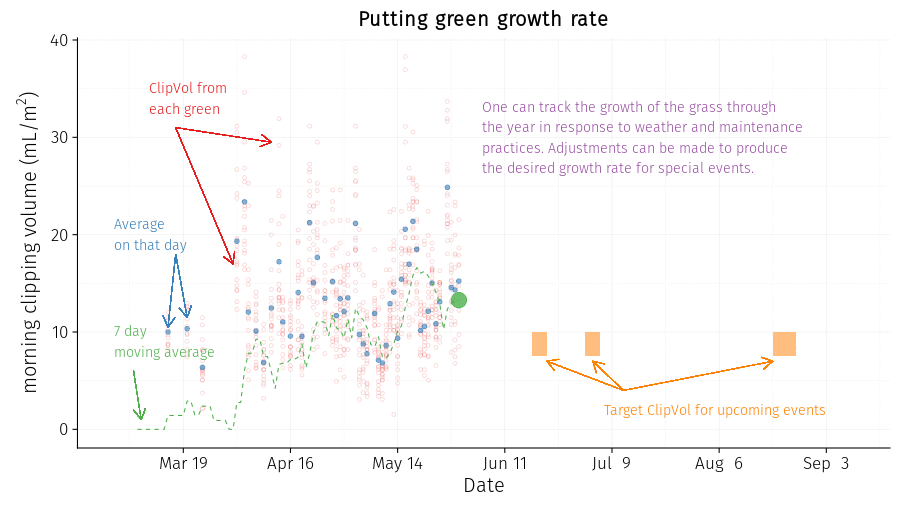
\includegraphics{img/y2018.png}
\caption{Annotated clipping volume chart with year-to-date clipping volume data as of early June}
\end{figure}

\begin{enumerate}
\def\labelenumi{\arabic{enumi}.}
\item
  I'll have some target growth rates for certain times of the year or for special events. I may also have some general targets for monthly and annual clipping volume. These targets will be based on previous measurements at my location.
\item
  I like to know the daily amounts and the variability from green to green. I look mostly at the daily average and may track the standard deviation among greens.
\item
  More than the daily amounts from any green, or the daily average of all measured areas, I like to look at a 5 day or 7 day moving average. For this average, I'll see how it compares to any upcoming targets. I'll also see if the slope (or trend) of the moving average is increasing or decreasing. Based on this, and a comparison to upcoming targets, and daily assessment of the grass conditions, I can make a lot of decisions about what maintenance work to do---or to not do---and how intensively to do certain works.
\end{enumerate}

\hypertarget{i-dont-really-need-any-data-for-this-to-be-certain}{%
\chapter{``I don't really need any data for this to be certain''}\label{i-dont-really-need-any-data-for-this-to-be-certain}}

Paul Robertson started a conversation\footnote{This chapter is an updated version of this post from 2017 (\url{https://www.blog.asianturfgrass.com/2017/06/i-dont-really-need-to-show-any-data-for-this-to-be-certain.html}). The conversation started as a simple inquiry about the Pelzmeter, and somehow ranged all the way to clipping volume.} on Twitter in 2017 that eventually touched on the quantity of clippings mown from the turf, how much the grass is growing, and the green speed. I was reminded of a question from a correspondent a few months ago. He wrote with this question:

\begin{quote}
``Have you correlated yield to speed? I have to assume that as yield changes speed changes also.''
\end{quote}

I replied:

\begin{quote}
"In the big picture view, yes the clipping volume will be negatively correlated with speed. When clipping volume goes up, the speed has to go down.
\end{quote}

\begin{quote}
I don't really need to show any data for this to be certain. Take, for example, warm-season greens. Are they faster when growing in August (clipping volume is a positive number), or when dormant in February (clipping volume is 0)? They are lightning in February and of whatever speed they are in August.
\end{quote}

\begin{quote}
I attach a chart with clipping volume in L/100 m2 (same as quarts per 1000 ft2) on the x axis and green speed on the y axis. That's from a couple years of tournament week measurements in Japan. Speed is affected by other things but the clipping volume is sure to have some effect and I don't think it will ever be in the direction of more growth = faster speeds.
\end{quote}

This is the chart I attached.

\begin{figure}
\centering
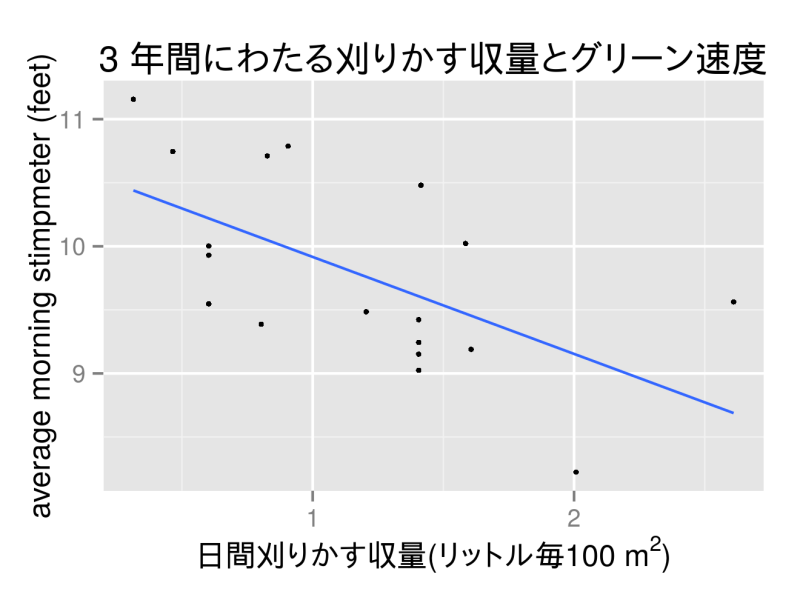
\includegraphics{img/b10-1.png}
\caption{This chart shows three years of paired clipping volume data from the 2013 to 2015 KBC Augusta tournament on the x-axis and average morning green speed on the y-axis}
\end{figure}

Today I looked up the data from 2016 and added it to the chart, and this includes a couple measurements from July 2016 a month before the tournament week.

\begin{figure}
\centering
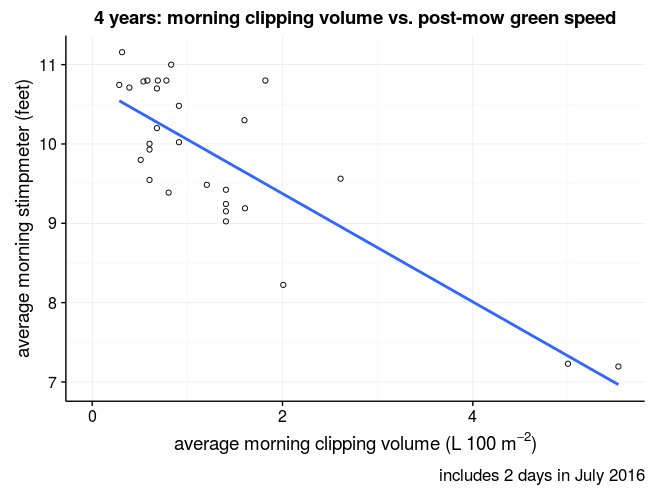
\includegraphics{img/b10-2.png}
\caption{Morning clipping volume and morning green speed at Keya GC}
\end{figure}

Here it is without the July measurements.

\begin{figure}
\centering
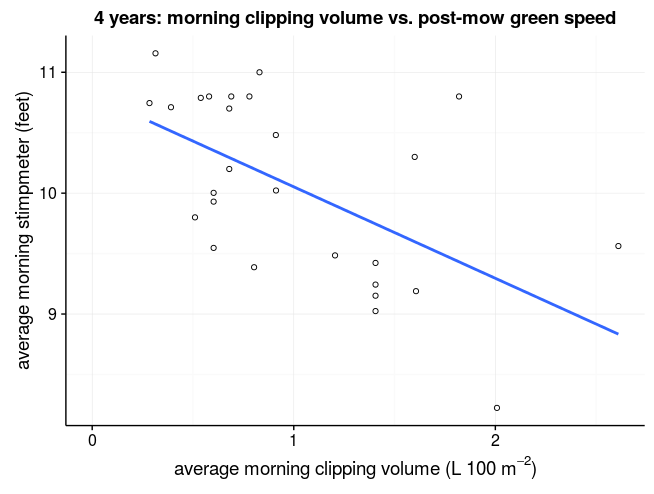
\includegraphics{img/b10-3.png}
\caption{Morning clipping volume and morning green speed at Keya GC, August only}
\end{figure}

And here are the data broken down by year.

\begin{figure}
\centering
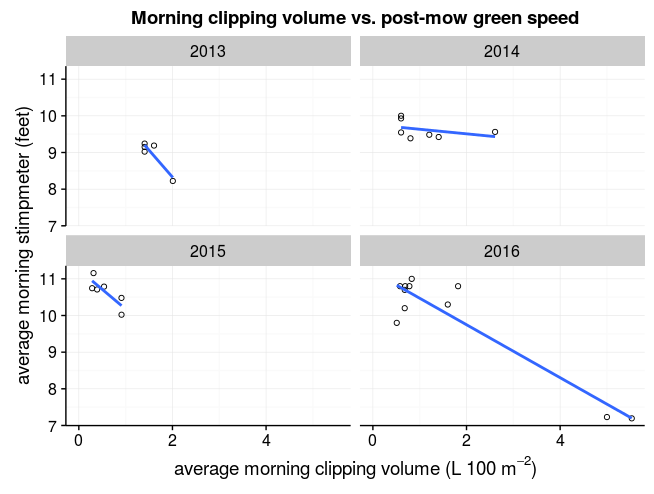
\includegraphics{img/b10-4.png}
\caption{Morning clipping volume and morning green speed at Keya GC facetted by year}
\end{figure}

Bill Kreuser showed data on bentgrass where the quantity of clippings was not related to the previous day's stimpmeter measurement. Those data (\url{https://twitter.com/UNLturf/status/879015787524104194}) are surely correct. But if one thinks about the big picture view, of the range of growth rates one can have over the course of the year, and the range of green speeds, I think it makes sense to think of green speed as being affected by how much the grass is growing.

And this leads me to something else that I can't help but mention. Bill can show data that demonstrate an interesting point; clipping yield was unrelated to green speed under the conditions of his experiment. I can show data that demonstrate an interesting point; clipping volume in the situation I describe is obviously associated with green speed. These experiments are not that hard to do; one could generate some kind of data about green speed and could make it show whatever one wanted to, if one planned it right, because \emph{there are a lot of factors that influence green speed!} So why is it so difficult to find data about Si and green speed? I still think it is ridiculous\footnote{\url{http://www.blog.asianturfgrass.com/2015/02/silica-and-green-speed.html}} that a stiffer leaf would make for a faster green speed.

\hypertarget{green-speed-again}{%
\chapter{Green speed again}\label{green-speed-again}}

The question of clipping amounts and their relation to green speed comes up frequently.

In general, the relationship between morning clipping volume and the green speed measured shortly after goes like this. When there are fewer clippings, the green speed is faster.

Of course, one can find plenty of exceptions. Three notable ones are here.

\begin{description}
\item[When one does a double cut, there will be more clippings, and the green speed will also be faster]
It might be useful to restrict direct comparisons to days on which the same work is done to the turf. But one can also express the clipping volume as per mow per day, rather than per day. Here's a quick description of this, with a background story. I've been most interested in clipping volume as a way to measure how much the grass is growing and how many nutrients the grass is using. Because of that, I want to know the total quantity of clippings removed, and I have reported the data in that way. I know a lot of people like to look at the relationship between clipping volume and green speed too. If one expresses the clipping volume as volume/area/mow, rather than volume/area/day, this relationship between clipping volume and green speed may be a little more obvious, especially in the case of double cuts. In that way, with a double cut, the volume is reduced by 50\%, and of course one expects the speed with a double cut to go up.
\item[When the turf is not mown every day,]
the speed will usually be faster on the day when it is mown and the clipping volume is \textgreater{} 0. Again, I find it useful to group the comparisons based on the work that was done.
\item[When the season is different,]
here will be inherent differences in the green speed that are related to plant morphology in addition to the effect of clipping volume.
\end{description}

This chart with data from 39 days of paired measurements at Keya GC in Fukuoka, Japan, shows all of these exceptions, and it also shows how one can expect clipping volume and green speed to be related.

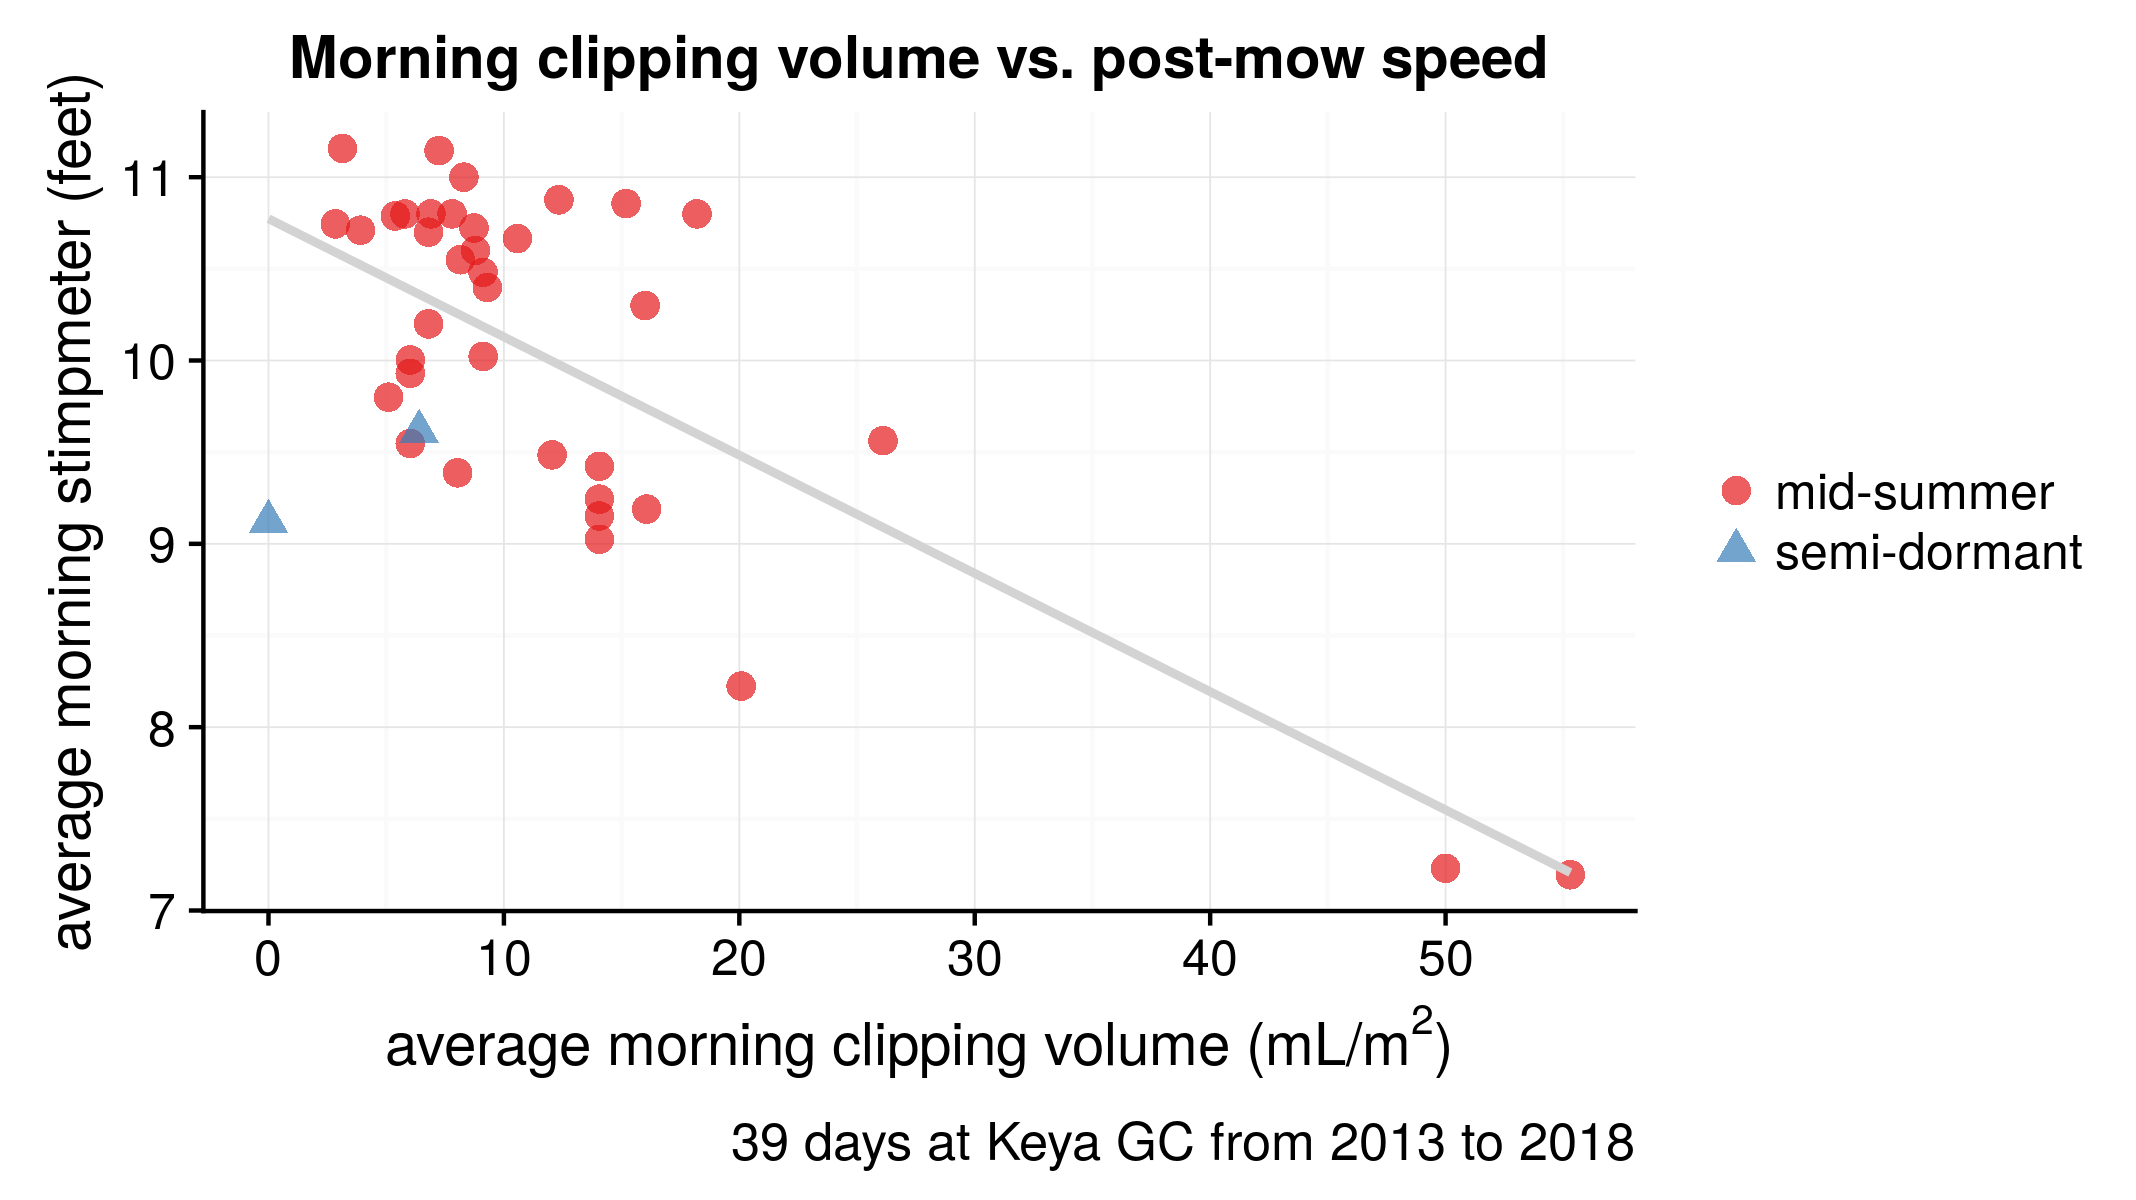
\includegraphics{img/clip_vs_speed.png}

The red circles are labeled ``mid-summer.'' They are all collected in July and August. Those two days at the bottom right were July 29 and July 31 of 2016, and represent the clipping volume with a single cut. 50 mL/m2 is a lot of clippings; the grass was growing fast on those days. You can imagine that if another cut had been put on the greens, the clipping volume may have gone up to 70 or 80---and the speed would have gone up too.

The blue triangles are from March 2018.\footnote{This chapter is modified from this post at the ATC site (\url{https://www.asianturfgrass.com/2018-03-25-clipping-volume-green-speed-and-units/}).} On March 24 the greens got a single cut and the clipping volume was 6 mL/m\textsuperscript{2}. On March 25 the greens were not mowed; the clipping volume was 0 and the speed was slower than the previous day when the clippings were more.

Over the course of days, months, and seasons, this is what I expect. If one were to do exactly the same work to the turf every day, then the relationship between clipping volume and green speed would be tighter.

\hypertarget{the-case-for-reactive-greenkeeping}{%
\chapter{The case for reactive greenkeeping}\label{the-case-for-reactive-greenkeeping}}

I've been sitting on this idea for a long time, and I decided April 1 would be a great day to write about it. You can decide if I'm serious.\footnote{I published the predecessor to this chapter on April 1---April Fools Day---in 2018. And I was and remain serious about this. Of course one must be proactive. But I think there is a great opportunity to improve turfgrass conditions, do less work, and have more fun doing the work, by adding a big dose of reactity to the work through a simple measurement of growth. Original post at \url{https://www.asianturfgrass.com/2018-04-01-is-reactive-better-than-proactive/}.}

When we first study turfgrass management, we tend to learn a proactive approach. This approach involves growing grass and regularly doing work such as fertilization, mowing, topdressing, and cultivation. These practices are generally done on a calendar schedule, albeit a flexible one, and are designed to be \emph{proactive}---from the OED, ``creating or controlling a situation by taking the initiative and anticipating events or problems \ldots{} innovative, tending to make things happen.''

Here's the problem. When we make things happen with the grass, we invariably overdo things. That's the only safe way to take a proactive approach. We don't know exactly what is going to happen with the weather, or with the grass conditions, so we must put a little too much fertilizer, proactively apply a little too much sand, and do a little too much aeration---remember we've added a little too much fertilizer already---and we must mow more than we otherwise would. This is more work. Can we get great turf conditions this way? Absolutely, but this is about making things happen with the grass and by all the extra work done, creating a surface.

Grant Saunders\footnote{You can find him on Twitter at \url{https://twitter.com/gslefty} or at the Hamilton GC maintenance page(\url{http://hamiltongcmaintenance.blogspot.com/}).} has asked a few questions over the past few years that have made me think this proactive approach may not be ideal.

First there was this one (\url{https://twitter.com/gslefty/status/573364242662883329}) about fertilizer: ``Stupid question time: Do you apply N to stimulate growth or is N applied in response to growth?''

One can think of this in two ways. Either apply N to cause growth, or think of the plant using N, and after some point it will require more, and then reapply when it does. The first approach is proactive, and the second is reactive.

Then there was this one (\url{https://twitter.com/gslefty/status/908912111098634240}) about sand: ``Have we become too precious about compaction? Firmness is good for the game. Producing surfaces vs growing grass.''\footnote{Check out these two links for some context. This was this discussion (\url{https://twitter.com/gslefty/status/908796355635699712}) and it was about the YouTube video (\url{https://youtu.be/r1LV77z_Ziw}) shared by Dan Dinelli about ball bounce on a fairway topdressed with sand, or topdressed with compost. Let's just say that the results might surprise you.}

When one can get better playing surfaces with less sand, why is the industry so proactive about applying sand?

And \emph{reactive} isn't such a bad word. From the OED, it means ``responds or reacts to a situation, event, etc., especially that reacts to existing circumstances, rather than anticipating or initiating new ones.'' Isn't that what one has to deal with in turfgrass management? Unpredictable weather, and grass that responds to weather just as much (or more!) as it does to any proactive greenkeeping? What if one was more reactive in responding to the grass and adjusting the work based on \emph{existing circumstances}. That sounds like an excellent approach.

I predict the reactive approach to greenkeeping produces equivalent or better turf conditions than a proactive approach, and does so with less work.

One way to be reactive? Measure how much the grass grows, from that estimate nutrient use and organic matter production, and react to existing circumstances.

\hypertarget{some-rise-some-fall-some-climb}{%
\chapter{Some rise, some fall, some climb}\label{some-rise-some-fall-some-climb}}

A full year of putting green clipping volume measurements looks like this.\footnote{This chapter is based on a blog post about what clipping volume is and how it looks over time. This is the post: \url{https://www.asianturfgrass.com/2018-06-10-some-rise-some-fall-some-climb/}.}

\begin{figure}
\centering
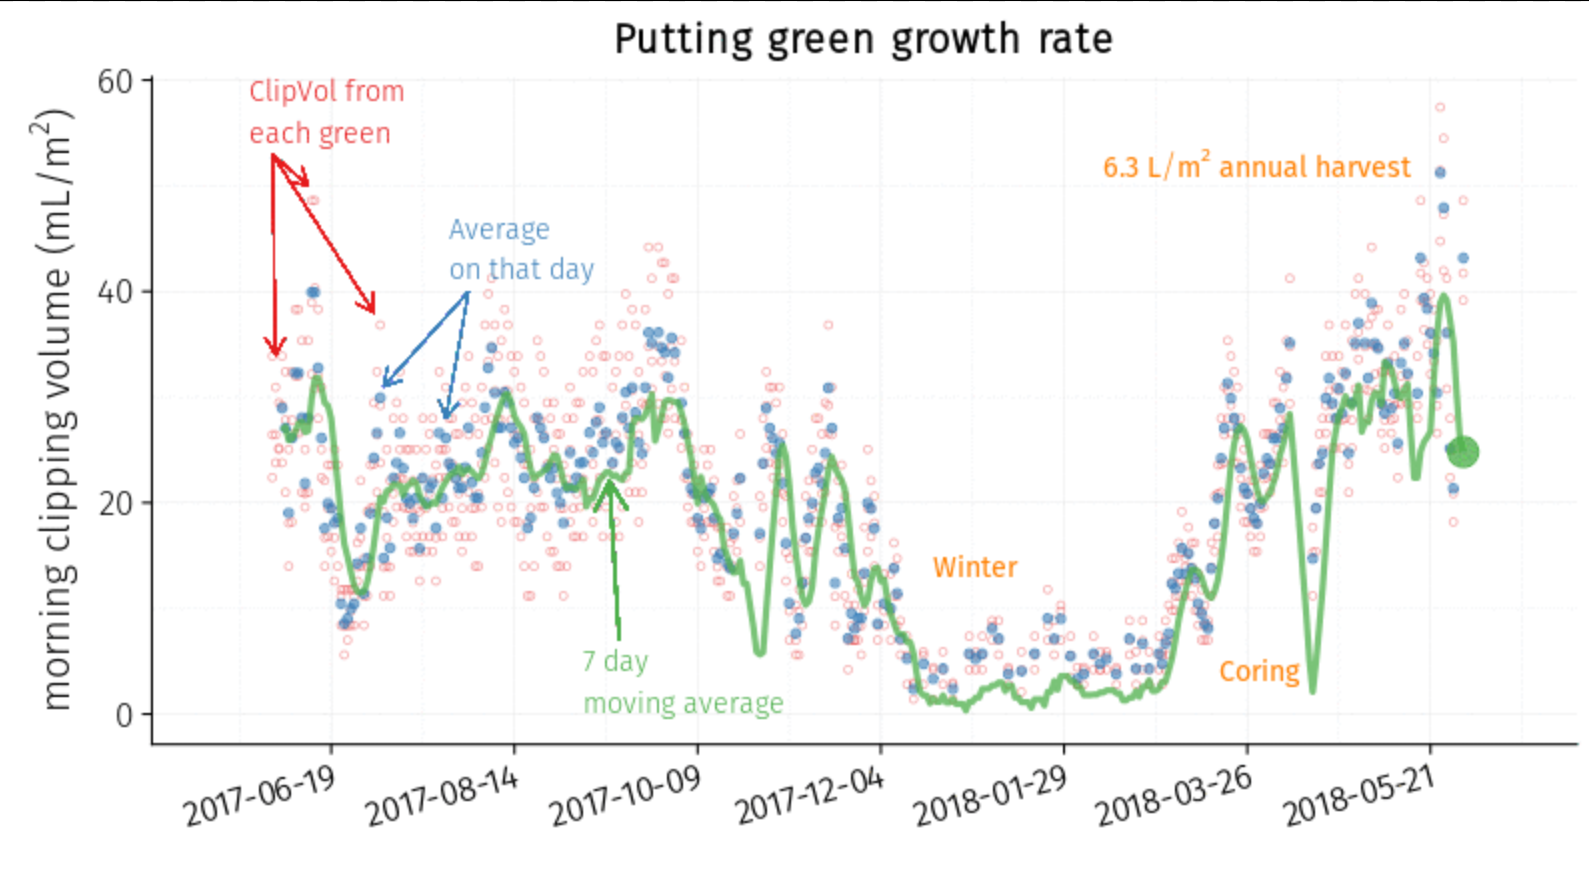
\includegraphics{img/b11-1.png}
\caption{Clipping volume for one year for seashore paspalum greens in northern Vietnam}
\end{figure}

Well, it's like that\footnote{An animated version of the chart above is available at this link: \url{https://c2.staticflickr.com/2/1751/28818470698_aaea9a9700_o_d.gif}} with a number of caveats. This is what it looked like:

\begin{itemize}
\tightlist
\item
  at this location 21° N latitude
\item
  with seashore paspalum turf
\item
  managed the way it was
\item
  with the weather of the past year
\item
  growing in the soil conditions of this site
\item
  irrigated with this water
\item
  etc.
\end{itemize}

I'd like to emphasize that the growth is in some ways out of the control of the turf manager, but the \emph{managed the way it was} category is a big one, and in that way the growth is adjusted, or even controlled, by the turf manager.

This is especially useful if one finds the optimum growth for one's site, and can then set a target for upcoming events, as was described in \protect\hyperlink{animation1}{the chapter on targets}

Three recent conversations, or things I've seen, are related to this.

First, a superintendent wrote to me, ``I \%\#!\&\^{}\% love \#ClipVol. What a useful tool it's been for us this season \ldots{} We'll mow tomorrow but I'll skip green 14 because of its slow growth rate. I also want to increase the growth rate so that's why I'm applying N tomorrow.''

That's good use of these data. I predict turf on 14 green will be better for not having been mowed, and of course applying N is going to move the growth rate closer to what this superintendent wants. With a number for the growth rate, it's easy to make these adjustments.

Second, Jon Merchant is measuring the clipping volume and finds the grass keeps on growing even more than desired, even with ``no N since May 4th'' (\url{https://twitter.com/Walsall_Greens/status/1004339720032309248}).

Here's a case where N applications seem to be delayed, skipped, or reduced in order to bring the growth rate to a desired level.

Third, Allan Dewald showed how temperature---and the associated increase in turfgrass growth potential---are ``interacting'' (\url{https://twitter.com/allan_dewald/status/1002037683189792774}) with clipping yields.

One can look at forecast temperatures and plan out fertilizer applications to hit the desired growth rates, and then make adjustments on the fly.

One can also adjust other things that will affect the clipping volume, such as growth regulators, soil water content, or rolling.

\begin{figure}
\centering
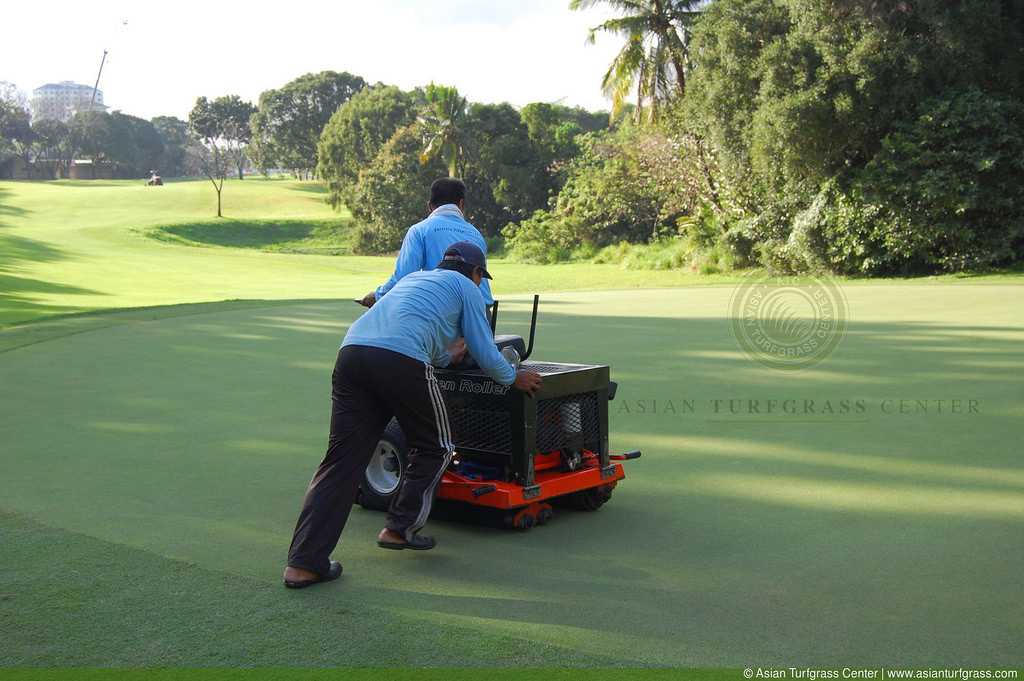
\includegraphics{img/b11-2.jpg}
\caption{A lightweight roller on a golf course putting green}
\end{figure}

One more thing---Allan made note of the double Y axis chart. That chart shows what he wanted it to show, although I'd like to think he was pointing the dual axes out as a disclaimer for the viewer. For more about the use of 2 y-axes, please see this \url{https://blog.datawrapper.de/dualaxis/}.

\hypertarget{predicting-organic-matter-in-turfgrass-soils}{%
\chapter{Predicting organic matter in turfgrass soils}\label{predicting-organic-matter-in-turfgrass-soils}}

Jason Haines has been sharing turf management ideas on his Turf Hacker (\url{https://www.turfhacker.com/}) blog, and one that I think is especially interesting is the idea that one can precisely match the topdressing sand quantity (\url{https://www.turfhacker.com/2018/06/sand-o-meter.html}) to the growth of the grass.\footnote{This chapter is based on a post I made about this topic on the ATC blog at \url{https://www.asianturfgrass.com/2018-06-29-predicting-organic-matter/}.}

I think this equation, or one similar to it, might predict what the soil organic matter content in turfgrass soils will be.

\begin{figure}
\centering
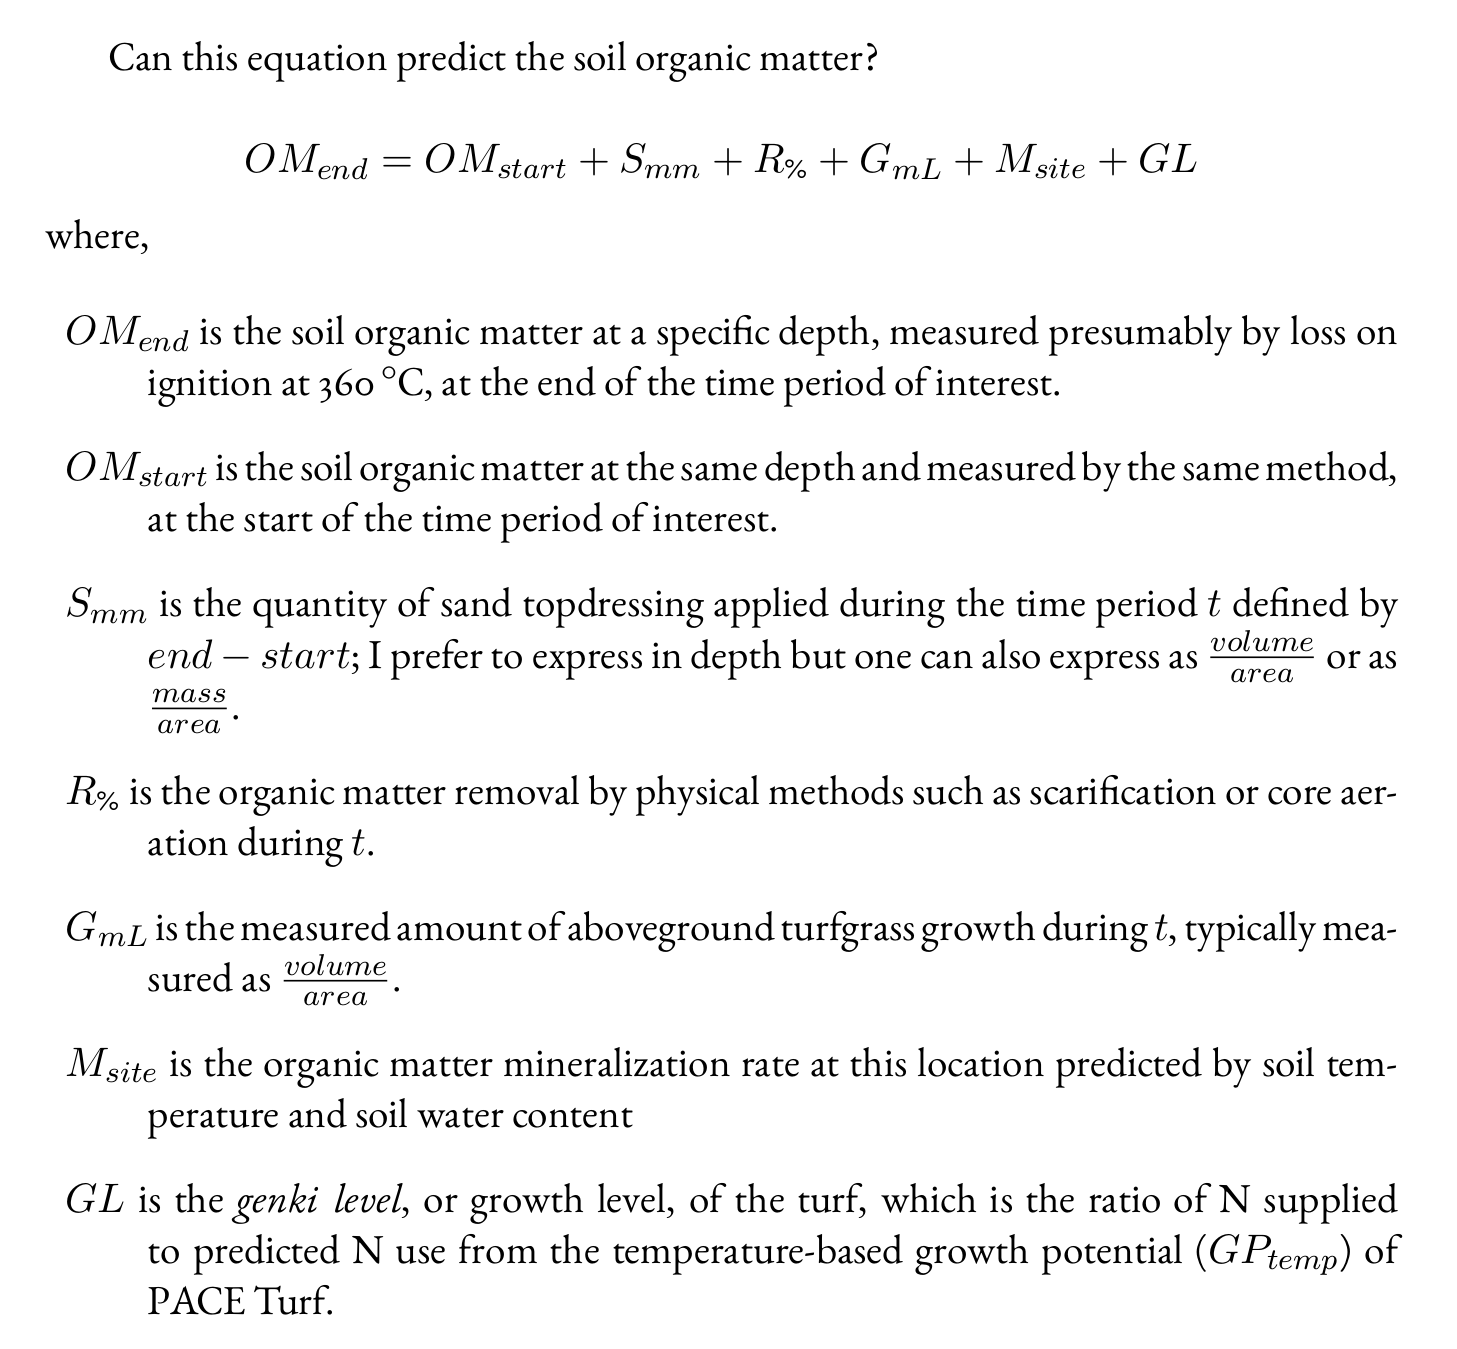
\includegraphics{img/om_prediction_equation.png}
\caption{Does this equation predict organic matter in turfgrass soils?}
\end{figure}

If that equation can predict soil organic matter, then it is relatively straightforward to adjust the variables on the right side of the equation in order to achieve the desired result on the left side.

And now for a different model! I've recently become aware of the \emph{Greens Organic Matter Management Tool} by Ed McCoy. You can read about this model and get an excel file to work with at this link:

\url{https://buckeyeturf.osu.edu/organicmattertool}

It is described as ``a location-based model of organic matter fate within the sand-based surface layer of a putting green.''

\hypertarget{hell-i-did-that-30-years-ago}{%
\chapter{``Hell, I did that 30 years ago''}\label{hell-i-did-that-30-years-ago}}

I enjoyed listening to my friends Dave Wilber and Kevin Ross in their TurfHead Jam Session (\url{https://www.turfnet.com/blogs/entry/1797-turfhead-jam-session-with-kevin-ross-session-number-1/}) number 1. They'd put out some teasers that they would be discussing ClipVol, so I made sure to listen as soon as the podcast came out, to see what these industry veterans had to say about that.\footnote{This chapter is based on this original post from September 2018 on the ATC website (\url{https://www.asianturfgrass.com/2018-09-29-did-that-30-years-ago/}).}

The section about clipping volume starts at 49:55, and they begin with lots of laughter and then these various observations:

\begin{itemize}
\tightlist
\item
  an American superintendent used metric units
\item
  is this busy work?
\item
  Kevin was doing this 30 years ago, back then they just called it ``clippings''
\item
  Kevin's given 8 or 10 presentations this year and only 1 person in the audience is doing this
\item
  older superintendents seem not to like this, in fact, one can really get them going (I assume this means in a bad way) if one would bring up clipping volume
\item
  they always knew what their clipping volume was, back in the day
\item
  they weren't desk jockeys when they were superintendents
\item
  it's all about playability
\end{itemize}

I appreciate that this is nothing new, that turf managers have \emph{always} and still do pay careful attention to how much the grass is growing, and that Dave and Kevin are supporting that focus, have always been interested in working things out, and they obviously realize that the amount of growth is important as it relates to playability.

But as I listened to them talk about clipping volume, I got the sense that they missed a few things, or perhaps haven't read much about \#ClipVol or seen how this is actually done.

I'd like to supplement what they said with a few things.

First, this is easy. It takes almost no time---this is a 10 second video showing the emptying of a basket into a bucket (\url{https://twitter.com/asianturfgrass/status/1032022780361895936}). In a lot less time than it takes to measure the soil moisture on a green, you can have a standard measure of how much the grass is growing.

And the units, whether in metric or whatever, can be forgotten if one likes. It works out to be a scale that goes from, in almost all normal grass growth situations, from 0 to 100.\footnote{I'll add that I recommend expressing in a standard unit for ease of communication. I find it really useful to be able to say, for example, that my Tifeagle greens or Penn A-4 greens had this much clipping volume in this much time when I did a certain amount of work. This is how I like to use the \emph{Grammar of Greenkeeping}, to express the work done and the conditions produced, and then to modify and make improvements. In order to do that, one uses a standard unit. But in reality, at any specific property, it works more like this. One know it is normal to get 12 L of clippings from the 5\textsuperscript{th} green. So does the person mowing that green. The manager, or the person operating the mower, gets a read on how much that turf is growing as soon as the basket is emptied. There is no desk jockeying or elaborate metric calculations. That stuff all happens automatically behind the scenes with some simply input of the total amount from each zone.}

Second, I'm not sure who was in the audience at Kevin's seminars this year. I also speak at a lot of seminars, and my experience has been that more people in the audience are measuring \#ClipVol than I expected.

Third, Dave and Kevin were doing this 20 and 30 years ago, paying attention to how many clippings they were getting. ``We always knew what our clipping yield was,'' they said. I understand that. But I think they would have trouble communicating what the clipping yield was to turf managers in another part of the county, let alone on the other side of the country or other side of the world.

Let's now jump ahead to right now, when two experienced turfgrass managers, consultants, and retired superintendents can sit down, record a podcast, and broadcast that all over the world to whoever wants to listen. That's awesome, it's a great time to be alive, and I love listening to how they did things back in the day.

Another great thing about the world today is that anyone can ask a question to essentially the world. For example, a superintendent in Oregon growing fine fescue could ask through TurfNet or Twitter for colleagues in Scotland also managing fine fescue greens, what are they doing to get the best conditions in terms of topdressing, fertilizer, irrigation, and by the way, what kind of clipping yield does that produce? They might even get an answer!

But there's a problem with knowing what your clipping yield is in terms of basket empties, or in general terms of growing a lot or not growing much, and actually expressing that as a number. I'm the only desk jockey I know of making tons of calculations and charts about this, so I've tried that measure of amount of clippings in the basket, or empties, and it just doesn't transfer. You can read all about that in \protect\hyperlink{report2014}{Appendix C} of this book.

If that growth number did transfer from site to site, just like other measures we use such as ET, soil temperature, mowing height, and so on, maybe turf managers from the younger generations could make good use of that. And just like a podcast can go out to the whole world, so also can questions or information about how much the grass is growing. This book introduces a lot of ways that the number can be used and there are plenty more that haven't been explored here.

No one has to measure the clipping volume. It's not necessary to measure clipping volume to produce good turf. But it is easy and it can lead to improved playing conditions with less work done to the turf. So I expect more and more people in the audience at Kevin's seminars to be familiar with this, or actually measuring clipping volume, in years to come.

\hypertarget{nothing-to-do-with-whether-or-not-it-works}{%
\chapter{``Nothing to do with whether or not it works''}\label{nothing-to-do-with-whether-or-not-it-works}}

Danny Vandecoevering (\url{https://twitter.com/DVturf}) wrote with this interesting email. I thought it was worth sharing here:\footnote{This chapter is reproduced with minor changes from this post on the ATC website (\url{https://www.asianturfgrass.com/2018-10-21-nothing-to-do-with-whether-or-not-it-works/})}

\begin{quote}
A couple weeks ago I asked you a question on twitter regarding what variation in day to day clipping volume would be considered statistically relevant. The reason I asked is because when I first heard about the concept of measuring clipping volume, my first thought was that there's no way that could be an accurate or consistent measure of growth. My thought at the time was that wet clippings would aggregate more than dry clippings, leading to higher volumes, or that a number of other factors would lead to information that wasn't consistent or useful. I don't think I was alone in thinking that at the time, and I'd bet many people still think along these lines. (For the record, I've made a complete 180 in terms of how I feel about collecting this data)
\end{quote}

\begin{quote}
What I find most interesting when I reflect on this early introduction to clip volume is not how I attempted to discredit its usefulness, but simply that I did. We apply water, in general, based on ET or what our moisture meters tell us. We apply pesticides and PGRs based on GDD models or other various environmental thresholds. Certainly, the same should apply to how we fertilize turf.
\end{quote}

\begin{quote}
I've been reading through a book called \emph{Thinking, Fast and Slow} (\url{https://www.amazon.com/gp/product/0374275637/ref=dbs_a_def_rwt_hsch_vamf_taft_p1_i0}) by a psychologist named Daniel Kahneman. The book discusses the tendencies of the conscious and subconscious human mind across many applications, and while dense, has been a fascinating read. The most recent chapter discussed the use of algorithms and formulas to make decisions versus the use of expert opinion. He discusses research done by Paul Meehl (specifically ``Clinical vs.~Statistical Prediction: A Theoretical Analysis and Review of the Evidence'' (\url{https://www.amazon.com/Clinical-Versus-Statistical-Prediction-Theoretical/dp/0963878492}) that has shown that 60\% of the time algorithms or formulas are a more accurate method of predicting an outcome than ``experts''. He then goes on to say that the remaining 40\% of the studies ended in a tie between experts and formulas, there were no examples of a human being a more accurate predictor than formulas and algorithms.
\end{quote}

\begin{quote}
He then goes on to say that this research is unsurprisingly unpopular among experts and specialists, and that the aversion to using algorithms or formulas to make decisions comes from humanity's deep - rooted desire for natural over synthetic.
\end{quote}

\begin{quote}
The topic of clipping volume kept coming to mind as I was reading this chapter, and I couldn't help but think that one of the greatest challenges to the widespread adoption of this method of greenkeeping has nothing to do with whether or not it works, but rather is contingent on one's ability to overcome their human nature. Meehl's research suggests that if one were to utilize clipping volume as tool to apply fertilizer then the worse case scenario is that the accuracy of their fertilizer applications doesn't improve or get better, but it is more likely that it improves.
\end{quote}

\begin{quote}
If you read all of this waiting for a question, sorry to disappoint, I simply thought the correlation between the research discussed in this book and the real life example of utilizing clipping volume to apply fertilizer was very interesting. I wouldn't be surprised to be sharing information you're already well aware of, but if not then I hope you find it interesting and / or helpful.
\end{quote}

\hypertarget{wrapping-things-up}{%
\chapter{Wrapping things up}\label{wrapping-things-up}}

There's sure to be a lot more information about this topic.

Joe Gulotti wrote ``Clipping volume, nothing to snicker at'' for \emph{Golfdom} magazine:

\url{https://www.golfdom.com/clipping-volume-nothing-to-snicker-at/}

I've talked with Doug Soldat and Bill Kreuser and I know they have been looking at these data in some detail. Their Greenkeeper App (\url{https://greenkeeperapp.com/}) also offers clipping volume data recording.

And there are a lot of turfgrass managers who are using clipping volume and getting good results and sharing information about that in various ways.

I've summarised most of what I've already written on this subject in this book. There's a bit of new information, supplemental information in the appendices hasn't been seen by many people, and this is my first attempt to put all this information about clipping volume together in one place. I hope you find this information useful.

\hypertarget{appendix-appendix}{%
\appendix}


\hypertarget{videos-and-slides}{%
\chapter{Videos and slides}\label{videos-and-slides}}

\hypertarget{recorded-presentations}{%
\section{Recorded presentations}\label{recorded-presentations}}

There is more information about clipping volume in presentation slides and videos.

The \emph{Leaves of Grass} video describes clipping volume measurements (\url{https://vimeo.com/micahwoods/clip1}). As I explained in the video description, the quantity of clippings mown from golf course putting greens can be quickly measured by noting the volume of the clippings. This gives an indication of the growth rate, and a number of management practices can be adjusted and optimized based on these data.

The TurfNet (\url{http://www.turfnet.com/}) webinar archive contains a recording of my presentation about \emph{Five reasons why you should measure the clipping volume}. It's a bit hacky to embed the video here, so watch it at this direct link, (\url{https://turfnet.wistia.com/medias/0tdfvy5qcr}), or find it on the TurfNet website. There are a lot of other good webinars to watch there too!

Here's what this TurfNet webinar was about:

\begin{quote}
Everyone checks the growth of the grass by counting basket empties or other more subjective evaluations of how rapidly the grass is growing. Measuring the volume of clippings mown from an area, and then reporting it as volume per area, is an exciting measurement that represents directly the overall objective of turfgrass management -- modifying the growth rate of the grass to create the desired playing surface.
\end{quote}

\begin{quote}
I shared data and case studies from around the world to explain how this measurement works and why the simple measurement of clipping volume has so many exciting implications for golf course maintenance. These include improved management (or optimization) of surface consistency, green speed, topdressing, and more.
\end{quote}

\hypertarget{slide-sets}{%
\section{Slide sets}\label{slide-sets}}

Here are a selection of slide sets that you can view online or can download.

\begin{itemize}
\tightlist
\item
  \emph{Turfgrass growth potential and measuring clipping volume} (\url{https://speakerdeck.com/micahwoods/turfgrass-growth-potential-and-measuring-clipping-volume}) from a presentation I gave in Lednice, Czech Republic, in December 2018.
\item
  \emph{Five reasons why you should measure the clipping volume}, the slides from the TurfNet webinar (\url{https://speakerdeck.com/micahwoods/five-reasons-why-you-should-measure-the-clipping-volume}).
\item
  \emph{Leaves of grass: applications and implications of clipping volume}, (\url{https://speakerdeck.com/micahwoods/leaves-of-grass-clipping-volume-from-putting-greens}), the slides from a presentation I gave in Moncton, Canada.
\end{itemize}

In these presentations, I generally express something like this:

\begin{itemize}
\tightlist
\item
  If one thinks of turf management as adjusting the growth rate, then it can be especially useful to know just what the growth rate is.
\item
  It doesn't take much time to measure the volume of clippings from putting greens. I used to think this was a silly measurement, but the particular case of preparing korai putting greens for tournament play quickly convinced me that these data are extremely useful.
\item
  There are a lot of other applications of this other than tournament preparation.
\item
  These applications can lead to improved turf conditions \emph{and} more efficient work.
\end{itemize}

I've discussed this in similar ways, or with portions of presentations focusing on clipping volume and the many ways the data can be put to use, in seminars over the past few years. You can find almost all my presentation slides at \url{https://speakerdeck.com/micahwoods}.

\hypertarget{june-2017-clipping-volume-report}{%
\chapter{June 2017 clipping volume report}\label{june-2017-clipping-volume-report}}

I prepared this progress report in June 2017 to share information with turf managers who shared clipping volume data with me over the past few years.\footnote{I want to say thank you again to everyone who has made the effort
  to collect the data and then the extra effort to share it with me.}

\hypertarget{introduction}{%
\subsection*{Introduction}\label{introduction}}
\addcontentsline{toc}{subsection}{Introduction}

I now have data on clipping volume from putting greens on nine golf
courses. For many of these courses there are data from multiple (or all)
greens at each mowing; for some of the courses there are data for a
selection of indicator greens, or for a single green. This report gives
a summary of the data collected so far, with some advice on how the data
can be understood and used, and with an explanation of what I'm trying
to learn from these data.

\begin{figure}
\centering
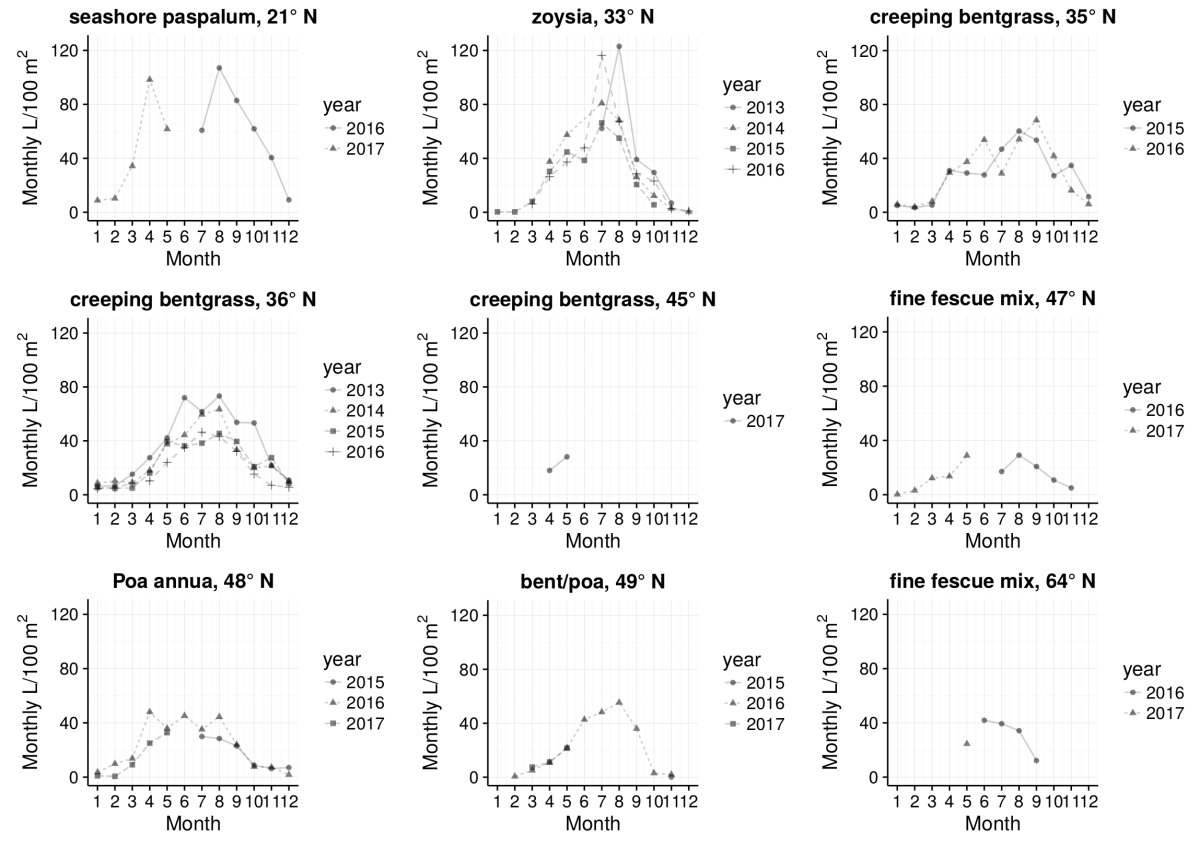
\includegraphics{figs/clip.png}
\caption{Clipping volume data from 9 locations as of May 2017}
\end{figure}

The previous page shows monthly totals for the nine locations.

\hypertarget{volHistogram}{%
\section{What's the use of clipping volume?}\label{volHistogram}}

In \emph{Short Grammar of Greenkeeping} I wrote that a way to define
greenkeeping is to say it is ``managing the growth rate of the grass to
create the desired playing surface for golf.'' The typical way to assess
growth rate is to observe the grass, and also to observe the quantity of
clippings. Because clippings from putting greens are collected in mower
baskets, it is a simple procedure to measure the volume of clippings as
the mower baskets are emptied.

I can think of many ways that these data might be useful, but the volume
data need to be put into context, or have some baseline comparisons,
before one can be confident in changing maintenance practices based on
them. Here's what I'm usually thinking of when I consider clipping
volume data:

\begin{figure}
\centering
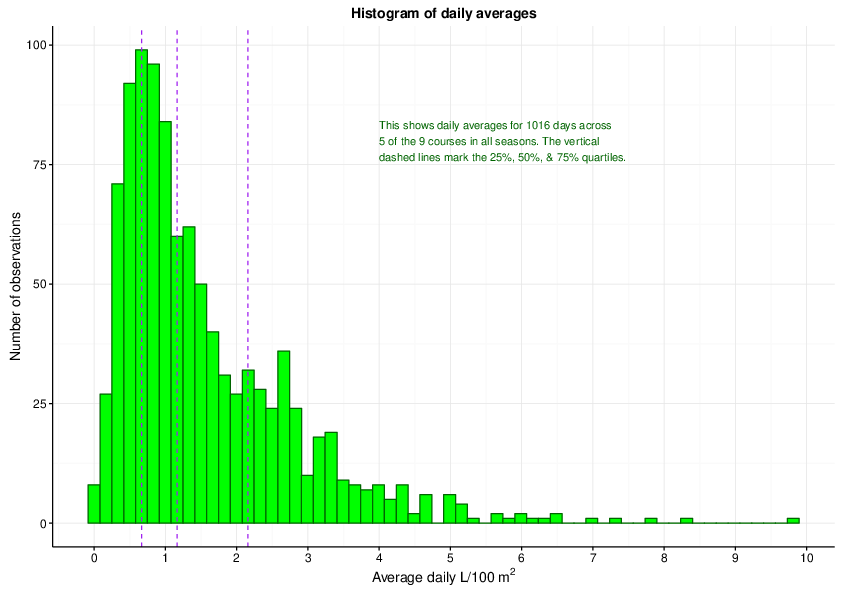
\includegraphics{figs/histDaily.png}
\caption{The median value for clipping volume is 1.2 L 100 m\textsuperscript{-2} and 50\% of the
measurements are from 0.67 to 2.2}
\end{figure}

\begin{description}
\item[growth rate tracking]
One might have a target growth rate for certain seasons, for
cumulative amounts to match traffic, or target rates for
special events. Big tournaments might have lower growth rates. Busy
seasons of golfing traffic might require faster growth rates. One
can compare from course to course, or one can compare within the
same course from year to year or season to season. I have been using
units of liters (L) of clippings per 100 m\textsuperscript{2} of green area. There
is plenty of variation, and that is normal. To pick the center of
the variation, I can describe the median values. When putting greens
are mown, the growth rate is such that 50\% of the time \textbf{the volume
is from 0.67 to 2.2, with a median of 1.2}. That's for all seasons
and doesn't correct for number of days since the last mowing. That's
just what is in the baskets, and the histogram in
Figure~1 shows what to expect. If you are getting
less than 0.67, then that is in the lower 25\%. That's not
much growth. And you might sometimes get from 2.2 up to about 10,
but that is rather high. This is not to say what any course \emph{should}
be, but is an attempt to put this into context.
\item[checking consistency or variability]
Are all greens growing at the same rate? Are all the mowers cutting
the same amount of grass? Is anything changing across the course as
a whole, or on a subset of greens? Having a number for the amount of
leaves being cut off the greens helps to answer those questions.
\item[adjusting inputs based on growth]
It seems reasonable in the day to day operations of a golf course to
consider making adjustments in the N supply, mowing height,
topdressing rate, growth regulators, rolling frequency, irrigation
rate, etc., based on how much the grass is growing and how much the
actual growth rate deviates from the desired growth rate.
\item[estimating the \emph{real} growth]
Volume is measured because it is easy. What can be even more useful
is the dry weight of the clippings harvested, but that is not
practical, for two reasons. First, one needs to separate any sand
collected in the clippings from the clippings themselves. Second,
one must dry the clippings in an oven. But one can make an estimate
of the dry weight from the clipping volume.
\item[estimating nutrient use and harvest]
Now we move on to topics that are of particular interest to me,
perhaps more from a research perspective rather than
turfgrass management. But if we have an estimate of the dry weight
harvest, then we can estimate nutrient removal through mowing on a
daily, weekly, monthly, and annual basis. If we know nutrient use,
then we should be able to match that with nutrient supply. We can
also compare locations. For example, if location X used this much N
and K and had a known growth rate, then location Y turf management
can be adjusted based on how location X was managed.
\item[topdressing and organic matter management]
Wouldn't it be nice to never topdress? To never core aerify? If the
surface conditions were perfect, and then the growth rate was 0, one
would never have to topdress or aerify. I am interested not so much
in eliminating topdressing or aerifying, but in trying to understand
how this work can be done as little, or as infrequently,
as possible. It seems likely that knowing the growth rate, and then
comparing what is done at location X and Y, one can get closer to
the objective of doing that work as infrequently as possible.
\item[checking temperature and growth potential]
When I first started looking into this, it was largely on
this topic. I was less interested in the actual amount of growth,
and was more interested in how it was related to temperature or
temperature-based growth potential. See, for example, this report
from 2014:
\url{http://www.seminar.asianturfgrass.com/20140612_clipping_yield.html}.
I'm less interested in that now -- more about that later.
\end{description}

In some of these areas, I have a pretty good idea of what the numbers
mean. In others, I don't, but I want to learn more and see if it is
possible to make use of the clipping volume data to get to an answer.
Here's a summary of where I'm at so far.

\hypertarget{growth-rate-tracking}{%
\section{Growth rate tracking}\label{growth-rate-tracking}}

I really started to get interested in these clipping volume data while
working with Andrew McDaniel at Keya GC during the KBC Augusta
tournament. I've written about this here:
\url{http://www.blog.asianturfgrass.com/2015/09/tournament-week-clipping-volume.html}.
To produce the desired putting surfaces for the tournament, it was
really helpful to check the clipping volume data. As I looked into this
more, I saw how easy it was to collect the data, and I realized that
there were a lot of uses for these data.

The second page of this report shows total amounts by month for
different grasses at different locations. From a look at that, you can
see what the normal amounts of clippings tend to be.
Figure~1 shows the clippings you can expect on a single
day. But of course that is bound to vary by season. I think it makes
sense to be familiar with the normal ranges and fluctuations at your
course, and also to know what is normal in the big picture of all
courses.

\begin{figure}
\centering
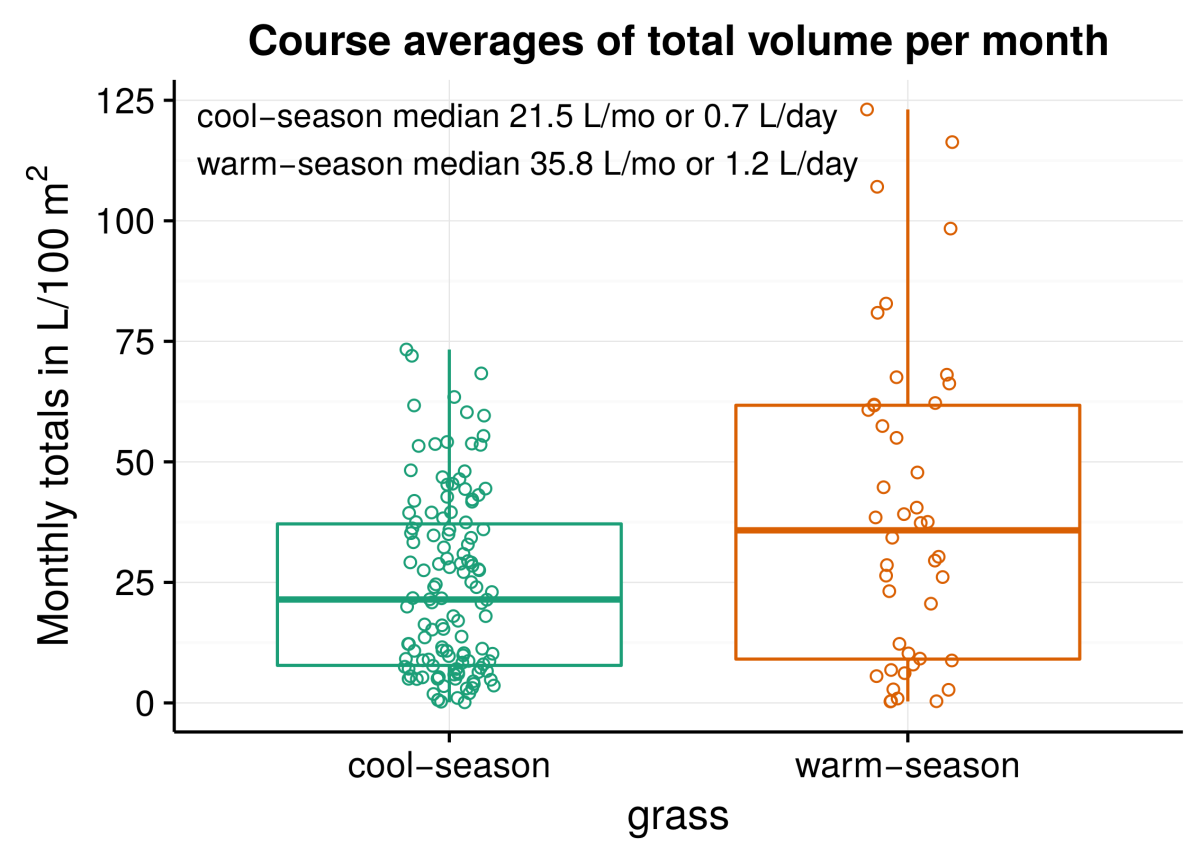
\includegraphics{figs/boxMo.png}
\caption{This boxplot shows the monthly totals for all nine courses. If one
divides the total volume in a month by the number of days in the month,
the result is an estimate of how much the grass is growing on a per day
basis.}
\end{figure}

Figure~2 shows the cool-season and warm-season monthly
totals. Remember, this is for all months, so it includes some months
when the grass is only mown a few times. But it generally represents
what is typical over a long period of time.

\hypertarget{checking-consistency-or-variability}{%
\section{Checking consistency or variability}\label{checking-consistency-or-variability}}

This is something I am really interested in. I know some places just
test one green, and use that to track some data. I find in most
interesting when all the greens are measured, because one can then check
that all mowers are cutting the same, and can evaluate the
microenvironments on the course that may influence growth, and can check
the consistency of the measurements.

I've spent a lot of time working on this, and don't have a perfect
answer yet. If you are really interested in this, please have a look at
\url{http://www.blog.asianturfgrass.com/2016/08/clipping-volume-variation-from-green-to-green.html}
and especially check the charts I showed in that post.

The best I can come up with now is this. When measuring all the greens
(or multiple greens), the median coeifficient of variation (CV) is about
0.33. The coefficient of variation is the standard deviation of all the
measurements, divided by the mean (average) of all the measurements.
That would be for a single day. If the CV is less than 0.33, you can
think of the greens as being more consistent than normal. If the CV is
more than 0.33, and as it moves above 0.4, then you can think the
clipping volume is less consistent than normal. The CV is not exactly
like going up or down by a fixed percentage, but I think it is
reasonable to look at it this way. If you measure say 18 greens, or 20
greens, or even 3 greens, and want to check the consistency, but don't
have an easy way to calculate the CV, \textbf{just take the average (mean) and
then go down 33\% and up 33\%. If all the clipping volumes are within
those boundaries, then the greens are more consistent than usual.} If
one or more greens are outside those boundaries, then the greens are
less consistent than normal.

I'm still working on this, so if you have suggestions, I'll be happy to
hear them. I prefer the coefficient of variation to describe the
variability in multiple numbers. I looked up the standard equation for
defining what is an \emph{outlier}, and that is 1.5 times the distance from
the 25\% quartile to the 75\% quartile. 50\% of the measurements will be in
that range, and one can take that range, multiply by 1.5, and then add
to the mean, and subtract from the mean, and then check if any
measurements are outside that range.

I prefer the CV to this outlier identification approach because I think
it more accurately represents what we would be looking at. Here's a
quick example with green speed to illustrate this.

Let's say we measure five greens with a stimpmeter. The greens have a
speed of 9, 9, 10, 11, and 11 feet. The average (mean) is 10 feet. The
standard deviation of those greens is 1 foot. That is, the average green
is 1 foot from the mean. The CV is then 0.1.

We could also have five greens with a speed of 9, 9.5, 10, 10.5, and 11
feet. Now the standard deviation goes down, because two of greens move
closer to the mean which remains at 10. The standard devation of those
five greens is 0.79 feet, and the CV is lower than 0.1; it is now 0.079.
The CV tells us something here. It shows which set of data have less
variation from the average value.

If we would take the outlier identification approach, it doesn't
identify any outliers.

\hypertarget{ajusting-inputs-based-on-growth}{%
\section{Ajusting inputs based on growth}\label{ajusting-inputs-based-on-growth}}

I don't have any numbers to share here, but if I were managing turf, I'd
be adjusting inputs based on how much the grass was growing. I'd look at
the grass, and I'd look at the color of the grass, and I'd check the
weather forecast, and I'd consider the current grass conditions and how
those compare to what I want the future grass conditions to be. To those
data or observations, I'd add the clipping volume data, and take these
all together to make better choices about what to do and what to change.
How to adjust the dials of the inputs to get the desired turfgrass
conditions, as Chris Tritabaugh has explained to me.

\hypertarget{estimating-the-real-growth}{%
\section{\texorpdfstring{Estimating the \emph{real} growth}{Estimating the real growth}}\label{estimating-the-real-growth}}

Volume is kind of useless. What we really want is dry matter harvest.
That is how much the grass grew, not counting water. How much actual
plant material was produced, per surface area of turf? While \emph{volume} is
useless, it is easy, and from volume we can estimate the dry matter
yield.

\hypertarget{fresh-weight-of-clippings}{%
\section{Fresh weight of clippings}\label{fresh-weight-of-clippings}}

I think volume is the easiest thing to measure. To measure fresh weight
one must bring along a scale, or bring the clippings back to a scale.
And then there is the issue of the water in the clippings, and the sand
in the clippings. Sand is going to affect the volume too, but I think
sand will have proportionately more effect on the mass of the clippings.

Andrew McDaniel\footnote{And the maintenance staff at Keya GC who have been so kind to
  bring a scale along with them on their 1, 6, 9 route.} has shared 2016 data with me of volume and fresh
weight measured from the same greens (Figure~3).

\begin{figure}
\centering
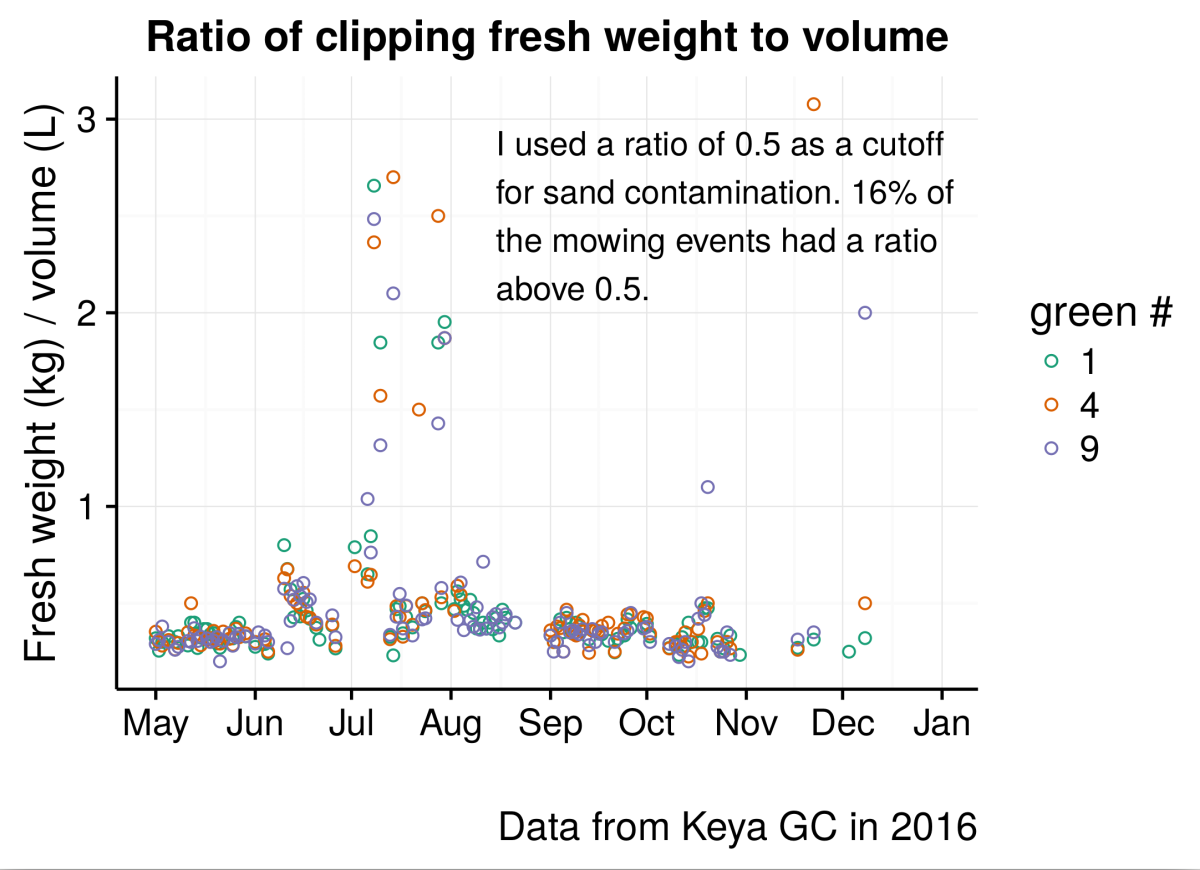
\includegraphics{figs/ratioChart.png}
\caption{The ratio of fresh weight to clipping volume for grass clippings
collected from three greens at Keya GC in 2016.}
\end{figure}

This is for korai greens, and the ratio may be different for other
species. But for korai, as Figure~3 shows, when the ratio of
mass to volume is more than 0.5, that is when there is a lot of sand on
the greens. These data are being collected again in 2017 at Keya. In
2016, 16\% of the mowing events had so much sand in the clippings that
the data had to be discarded, if we use that 0.5 ratio cutoff rule.

But after getting rid of the samples that are contaminated with sand,
there is a consistent relationship between fresh weight and volume
(Figure~4). To reiterate, \textbf{I prefer to measure clipping
volume because volume is easier to measure, and because volume has less
of a problem with sand mass error.} And after one has measured volume,
one can predict the mass anyway.

\begin{figure}
\centering
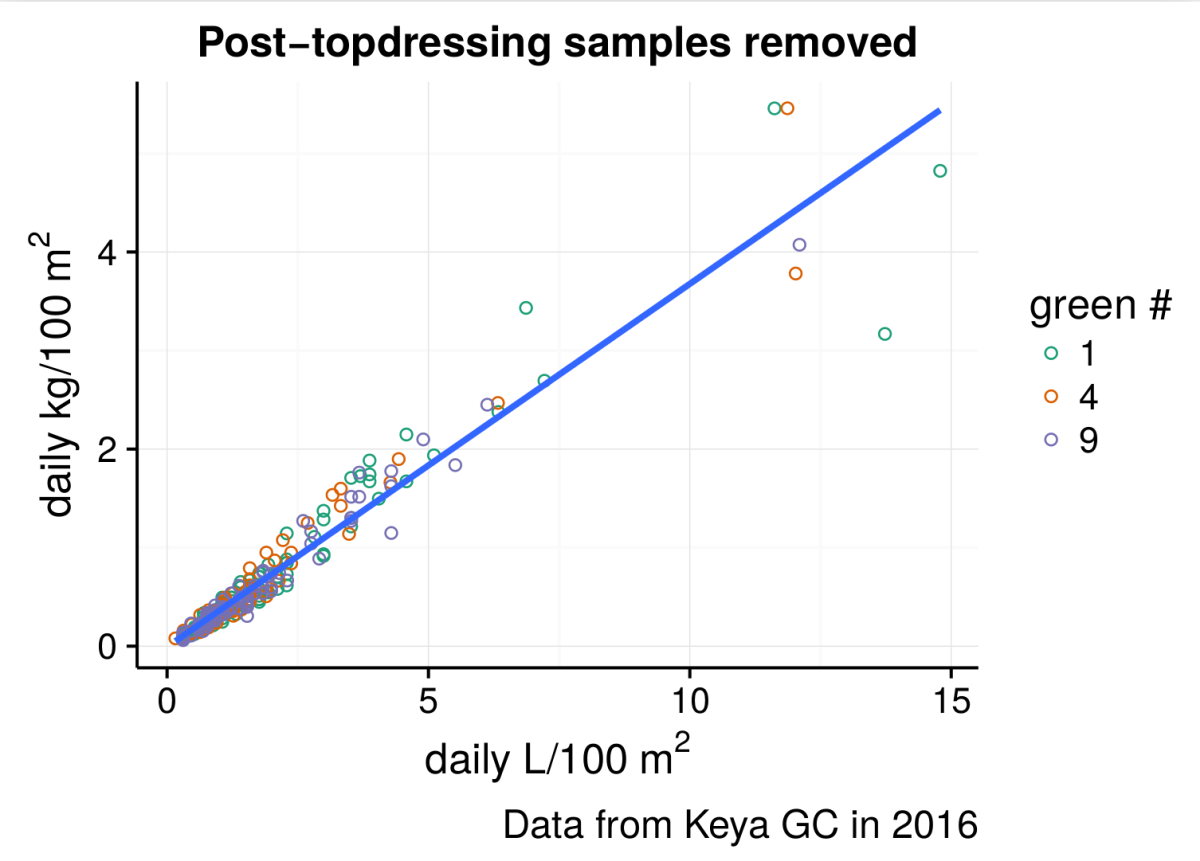
\includegraphics{figs/volTokg.png}
\caption{The clipping volume has a consistent relationship to the fresh weight
of the clippings when sand-contaminated samples are removed.}
\end{figure}

\hypertarget{estimating-nutrient-use-and-harvest}{%
\section{Estimating nutrient use and harvest}\label{estimating-nutrient-use-and-harvest}}

This is something I find really interesting. If we can estimate the dry
matter harvest from the clipping volume, then we can have an idea of how
many nutrients the grass is using. Mr.~Kihara and Mr.~Seiyama from
Nichino Ryokka carefully collected clippings and measured volume, fresh
weight, and dry weight at the Nichino Ryokka research center in Chiba.
Figure~5 shows the relationship between clipping volume
and clipping dry weight (there is a drying oven at the research center)
for three different grasses.

\begin{figure}
\centering
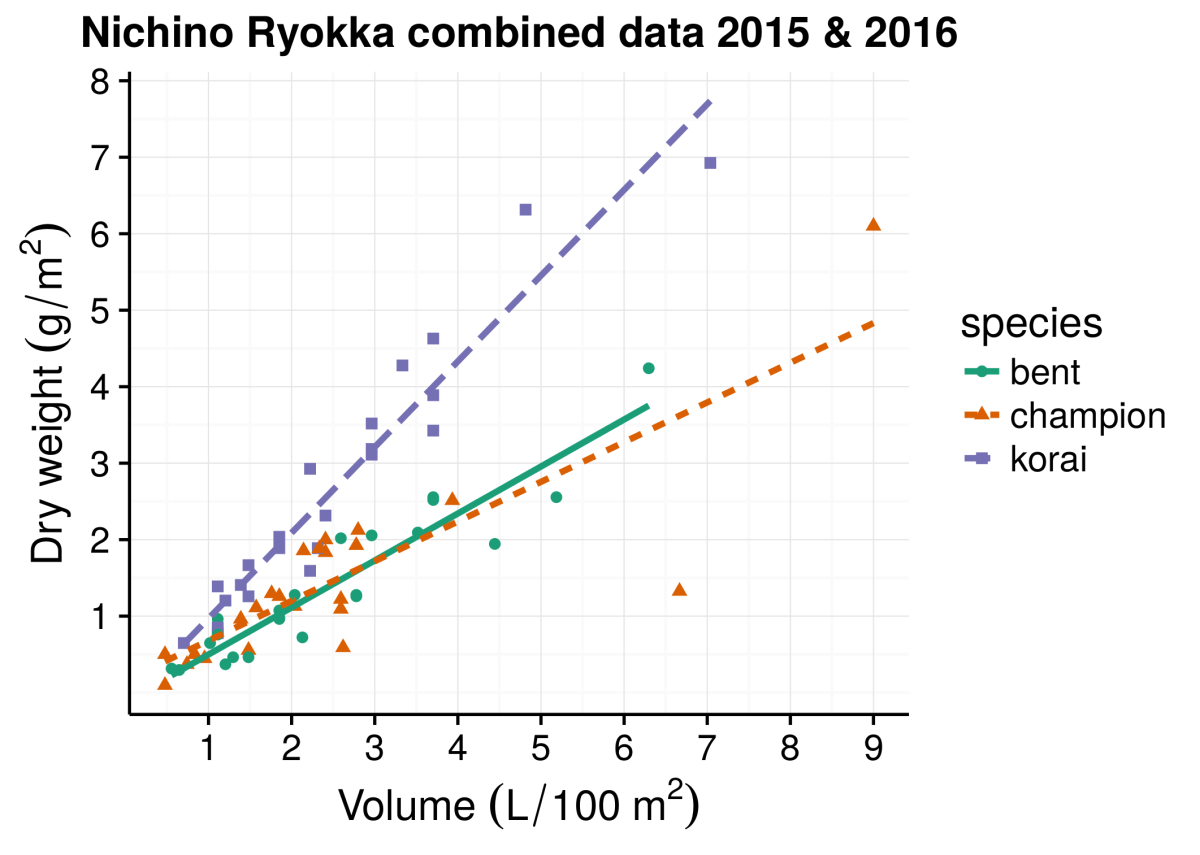
\includegraphics{figs/dryWeight.png}
\caption{Data from the Nichino Ryokka research center show that dry weight of
grass clippings can be predicted based on the clipping volume}
\end{figure}

If we focus on creeping bentgrass and \emph{Zoysia matrella} (korai), I'll
quickly explain how this works. First, let's do bentgrass. The slope of
the line (in Figure~5) for the bentgrass volume to dry
weight relationship is 0.63 g m\textsuperscript{-2} for every 1 L 100 m\textsuperscript{-2}. The
bentgrass greens at the location 36 degrees North latitude have an
average annual yield in volume of 326 L 100 m\textsuperscript{-2}. That works out to an
expected annual clipping harvest of 205 g m\textsuperscript{-2}. If the bentgrass leaves
have 4\% N, that is 8.2 g N m\textsuperscript{-2}. The N applied to those greens in 2014
was 12.9 g, then 10.1 in 2015, and I don't have the final numbers for
2016 but it was less than 10. So there seems to be a pretty close
correspondence between the N applied and the growth.

For korai, I'll use the data from the zoysia at 33 degrees North. The
average clipping volume from 2013 to 2016 at this location was 340 L 100
m\textsuperscript{-2}. From the Nichino Ryokka data, we can expect each liter of korai
clippings in 100 m\textsuperscript{2} to work out to 1.1 g of dried clippings in 1 m\textsuperscript{2}.
That gives an expected harvest of 374 g m\textsuperscript{-2}, and if the korai
clippings have 3\% N, that would be a N harvest in the clippings of 11.2
g m\textsuperscript{-2}. At this location, the N applied from 2013 to 2016 was 14.6,
9.5, 10.6, and 11.1 g m\textsuperscript{-2}. We can work through this for every element.
I just show for N to point out that in the case of profesionally-managed
turf (both the bentgrass and korai course used as examples here host
professional tournaments too) supplied with a relatively low amount of N
fertilizer, the quantity of clippings produced is related to the
quantity of N supplied.

\textbf{The implications of this are that one can be more precise in nutrient
applications.} And I am interested in this as a way to check nutrient
depletion rates from the soil, and do some calculations related to the
\textsc{MLSN} guidelines. I think
for most turfgrass managers, it is enough to understand that the
clipping harvest represents a quantity of nutrients, and also the
fertilizer applied represents a quantity of nutrients. This particular
aspect is more of a research thing, rather than a turf management thing,
but I am especially interested in this.

You can imagine what I think of supplying two or three or more times the
quantity of an element, like potassium or phosphorus or calcium,
compared to the amount that is used by the grass. These calculation are
a way to document this.

\hypertarget{topdressing-and-organic-matter-management}{%
\section{Topdressing and organic matter management}\label{topdressing-and-organic-matter-management}}

But this growth, as it relates to the nitrogen supply, is quite
pertinent to this section. I don't have too much to say here, other than
it makes sense to me that if the grass grows less, by less N supply,
then there will be less of a need for topdressing and core aeration.

If you haven't, see
\url{http://www.blog.asianturfgrass.com/2016/05/data-to-support-an-anecdote.html}
for more about this. This is about a course doing 45,000 rounds per year
and that has dormant grass for 6 months. The N supply is low, the grass
conditions have gotten better year after year, and the soil organic
matter keeps going down. But the core aeration and topdressing are also
less than what you might expect.

I believe this approach can be implemented in more places. And I think
measuring clipping volume can be a way to compare locations. So if X
location is having great success with this much topdressing and this
much N and this much clipping volume, I think the clipping volume
comparison from place to place can be used to fine tune some of the
organic matter management. I've written articles about this in my series
for \emph{Golf Course Seminar} magazine, in particular I think the March and
April 2017 issues. When I get the 2\textsuperscript{nd} edition of \emph{Short Grammar of
Greenkeeping} to the printer, those articles (in English) will be
included as appendices.

\hypertarget{checking-temperature-and-growth-potential}{%
\section{Checking temperature and growth potential}\label{checking-temperature-and-growth-potential}}

This was my original interest in this, and I am still working to
understand this. There is obviously a relationship -- look for example at
seashore paspalum at 21 degrees North -- it grows less in winter. Look at
fine fescue mix at 64 degrees North -- it doesn't grow in winter. At the
broad scale, temperature plays a huge role. Actually, looking at all the
charts again, it is easy to see how much of a seasonal -- a temperature --
effect is there.

As I've become interested in predicting dry weight of clippings and
nutrient use of grass, and also trying to understand what normal
variability of growth is, I put the temperature analysis on the back
burner. I'm still really interested in this, but there is only so much
time to work on it!

\hypertarget{report2014}{%
\chapter{Looking at clipping yield from putting greens}\label{report2014}}

Some golf course superintendents take a measure of clipping yield at each mowing.\footnote{This was a report I put together in June 2014. You can find it at (\url{http://www.seminar.asianturfgrass.com/20140612_clipping_yield.html}).} I wanted to look at those data for these reasons:

\begin{enumerate}
\def\labelenumi{\arabic{enumi}.}
\tightlist
\item
  to see how yield is affected by temperature
\item
  to see how yield is affected by growth potential (GP)
\item
  to see if GP assumptions in growth can be detected by combining data from multiple sites
\end{enumerate}

Golf course superintendents shared data with me from 5 locations:

\begin{enumerate}
\def\labelenumi{\arabic{enumi}.}
\tightlist
\item
  Canada, cool-season grass
\item
  Japan, warm-season grass
\item
  Japan, cool-season grass
\item
  New Zealand site 1, cool-season grass
\item
  New Zealand site 2, cool-season grass
\end{enumerate}

What I've done here is rough, but I find it quite interesting. Please keep these things in mind when looking at the results:

\begin{itemize}
\tightlist
\item
  Measurements were in different units. Liters per green, liters per green reported on a 100/m\^{}2 basis, and number of time the baskets were emptied per mowing event.
\item
  I've adjusted these measurements to a scale of 0 to 1, by dividing each measurement by the maximum measurement at that site. That gives fraction of the maximum clipping yield.
\item
  For the sites in Japan that measured the number of liters per day, I smoothed the measurement by taking the average of today's yield and the yield on the previous 4 days.
\item
  For one location I used on-site temperature data; for other locations I looked up the closest daily weather data I could find.
\item
  I did not make any effort to account for N applications, growth regulator applications, irrigation, or verticutting or topdressing or other maintenance practices that may influence yield.
\item
  I removed some outliers of exceptionally high clipping yield from a couple sites.
\item
  My guess is that with data from enough sites, there would be a general trend in clipping yield in response to temperature or GP, averaged across all the sites, that would cancel out all the noise from the day-to-day variability in maintenance practices that influence yield.
\end{itemize}

Charts by location

These plots look at the GP and the yield, both on a scale of 0 to 1, across time, on a site by site basis. I wanted to see how the clipping yield was related to the GP. For the warm-season grass in Japan, the clipping yield and the GP track pretty closely, more so than the clipping yield and the temperature.

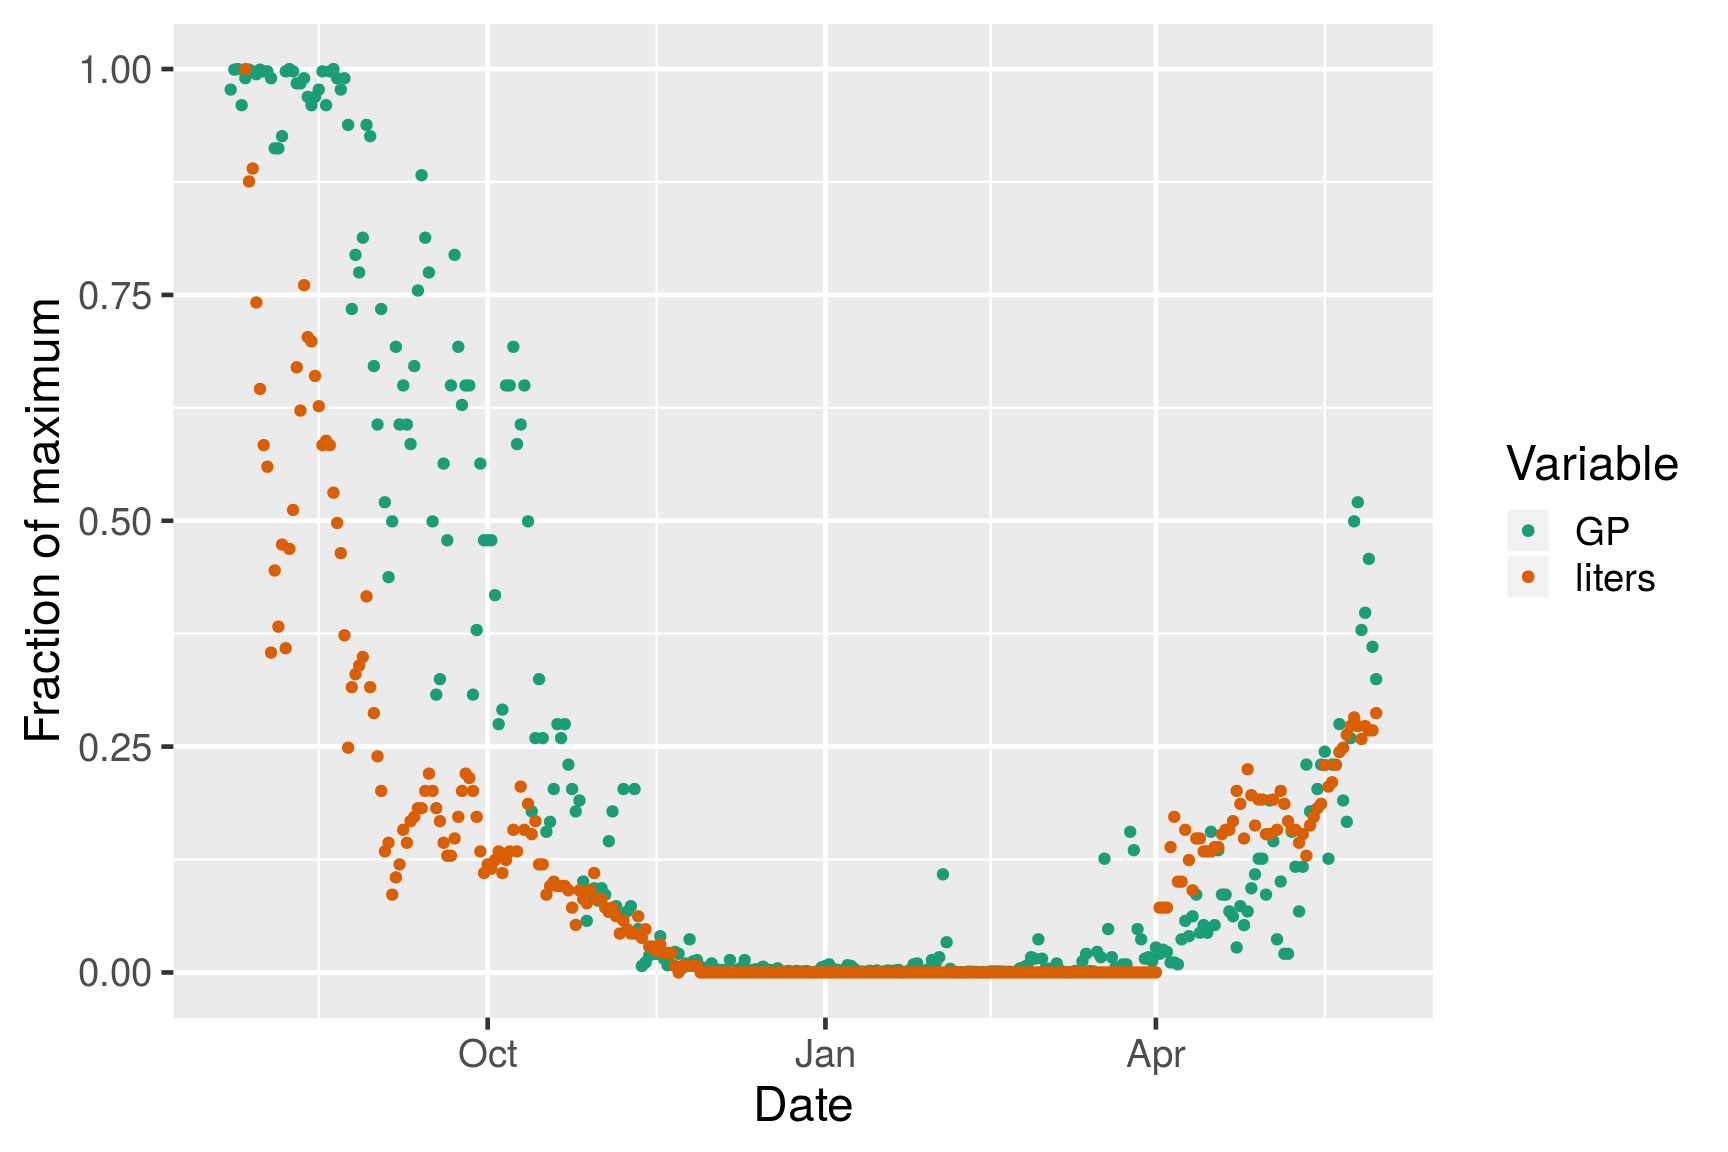
\includegraphics{clip_book_files/figure-latex/keya1-1}
\includegraphics{clip_book_files/figure-latex/keya1-2}

For cool-season grass in Japan, the GP and the yield have a similar trend, but the yield tracks with temperature even more cleanly.

\includegraphics{clip_book_files/figure-latex/ohtone-1}
\includegraphics{clip_book_files/figure-latex/ohtone-2}

These charts show the yield over time and the GP and the temperature at the Canada site; note that the data now are number of basket empties per day.

\includegraphics{clip_book_files/figure-latex/canada1-1}
\includegraphics{clip_book_files/figure-latex/canada1-2}

For New Zealand, the data are similar between sites. These charts show the yield, again in empties per day, plotted with GP and with temperature.

\includegraphics{clip_book_files/figure-latex/nz1-1}
\includegraphics{clip_book_files/figure-latex/nz1-2}

I think it is interesting to look at the relationship between GP and yield for all sites together. This is a bit messy.

\includegraphics{clip_book_files/figure-latex/all-1}

Looking at the fraction of maximum yield for all locations actually makes more sense when plotted by temperature.

\includegraphics{clip_book_files/figure-latex/alltemp-1}

My thoughts at this point:

\begin{enumerate}
\def\labelenumi{\arabic{enumi}.}
\item
  Measuring in liters (volume of clippings) is a bit more precise than empties per day. If this were to be a larger project from multiple locations, it would be nice to have those cleaner data.
\item
  The yield of bentgrass in Japan doesn't drop much even when temperatures are well above the optimum. For the cool-season grasses at Canada and New Zealand, the temperatures didn't get much above the optimum (20°C). Maximum yield was seen even at less than 15°C.
\item
  The data that match GP best are for warm-season grass at Japan. I think this is because the optimum temperature is always higher than the actual temperature. For cool-season grass, the optimum growth can occur across such a wide range of temperatures, and this makes the data messier for cool-season.
\item
  Even if these charts look messy, and there is not a clear relationship between GP and yield, I like GP. It gives a number in the range of 0 to 1, which is useful in a number of ways, it is \emph{potential}, not \emph{reality}, and it gives a warning when temperatures move away from the optimum in a way that linear representations of temperature does not.
\end{enumerate}

\hypertarget{even-more-information}{%
\chapter{Even more information}\label{even-more-information}}

If you just can't get enough of this type of information, then please do the following.

First, check \url{https://www.asianturfgrass.com/} regularly. I keep it updated with new turfgrass information and ideas.

Second, please subscribe to one of the ATC newsletters at \url{https://www.asianturfgrass.com/lists/}. You can browse that page to find the newsletter/s that are of interest to you, and then sign up.

Third, see these books: \url{https://www.asianturfgrass.com/books/}.

Fourth, see the footer (the very bottom of the page) at the ATC website (\url{https://www.asianturfgrass.com/}) for our email and all the ATC social media or online accounts. Please connect with us to get more information.

\bibliography{/home/micah/Documents/Rs/citations.bib}



\end{document}
